% ======================================================================
% Informe — Torneo FEN–Banco Itaú "¿Sube o baja el dólar mañana?"
% Compilar con pdfLaTeX (Overleaf). Subir a la misma carpeta:
%   escudo1.pdf · curva.png · curva_holdout.png (salen de estrategia.py)
%   fig_detector_pasos.png · fig_detector_galeria.png      (exp 14)
%   fig_sensibilidad.png (exp 15) · fig_placebo.png (exp 16) · fig_correlaciones.png (exp 17)
% Si falta una figura, el documento compila igual y muestra un recuadro.
% \completar{...} (rojo) = dato pendiente. Buscar "completar" antes de entregar.
% ======================================================================
\documentclass[10pt,a4paper]{article}
\usepackage[utf8]{inputenc}
\usepackage[T1]{fontenc}
\IfFileExists{spanish.ldf}%
  {\usepackage[spanish,es-nodecimaldot,es-noshorthands,es-tabla]{babel}}%
  {\AtBeginDocument{\renewcommand{\figurename}{Figura}\renewcommand{\tablename}{Tabla}%
   \renewcommand{\abstractname}{Resumen}\renewcommand{\appendixname}{Apéndice}}}

% ---------- Página y tipografía ----------
\usepackage[a4paper,top=2.5cm,bottom=2.3cm,left=2.4cm,right=2.4cm,headsep=0.8cm]{geometry}
\IfFileExists{lmodern.sty}{\usepackage{lmodern}}{} % monoespaciada (código)
\usepackage[sc]{mathpazo}            % Palatino para texto y matemática
\usepackage[scaled=0.90]{helvet}     % Helvetica para títulos
\linespread{1.06}
\usepackage{microtype}
\setlength{\parindent}{0pt}
\setlength{\parskip}{5pt plus 1pt}

% ---------- Paquetes ----------
\usepackage{booktabs,tabularx,multirow,array}
\usepackage{graphicx}
\usepackage{amsmath,amssymb}
\usepackage{enumitem}
\usepackage{tikz}
\usepackage{xcolor}
\usepackage{float}
\usepackage[section]{placeins}       % las figuras no saltan a otra sección
\usepackage{titlesec}
\usepackage{tcolorbox}
\usepackage[round,authoryear]{natbib}

% ---------- Colores ----------
\definecolor{azul}{HTML}{0B2A5B}
\definecolor{azulclaro}{HTML}{E9EEF6}
\definecolor{gristexto}{HTML}{4A4A4A}

\usepackage[colorlinks=true,linkcolor=azul,citecolor=azul,urlcolor=azul]{hyperref}

% ---------- Títulos de sección ----------
\setcounter{secnumdepth}{2}          % se numeran secciones y subsecciones
\titleformat{\section}{\sffamily\Large\bfseries\color{azul}}{\thesection}{0.7em}{}%
  [\vspace{-4pt}{\color{azul!35}\titlerule[0.8pt]}]
\titleformat{\subsection}{\sffamily\large\bfseries\color{azul}}{\thesubsection}{0.6em}{}
\titleformat{\subsubsection}{\sffamily\normalsize\bfseries\color{azul!85!black}}{}{0em}{}
\titlespacing*{\section}{0pt}{16pt plus 3pt minus 2pt}{8pt}
\titlespacing*{\subsection}{0pt}{12pt plus 3pt minus 2pt}{4pt}
\titlespacing*{\subsubsection}{0pt}{9pt plus 2pt minus 2pt}{2pt}

% ---------- Leyendas ----------
\usepackage{caption}
\captionsetup{font={small,color=gristexto},labelfont={bf,sf,color=azul},
  labelsep=period,margin=0.5cm,skip=6pt}
\captionsetup[table]{position=bottom}

% ---------- Listas ----------
\setlist{itemsep=2pt,topsep=3pt,parsep=0pt}

% ---------- Ubicación de figuras y tablas ----------
\renewcommand{\topfraction}{0.85}
\renewcommand{\bottomfraction}{0.6}
\renewcommand{\textfraction}{0.12}
\renewcommand{\floatpagefraction}{0.8}
\setcounter{topnumber}{3}
\setcounter{bottomnumber}{2}
\setcounter{totalnumber}{4}
\setlength{\textfloatsep}{14pt plus 2pt minus 4pt}
\setlength{\floatsep}{12pt plus 2pt minus 2pt}

% ---------- Recuadros ----------
\newtcolorbox{ideaclave}{colback=azulclaro,colframe=azul,boxrule=0pt,leftrule=3pt,
  arc=0pt,outer arc=0pt,left=8pt,right=8pt,top=5pt,bottom=5pt,
  before skip=6pt,after skip=10pt,fontupper=\small}
\newtcolorbox{recuadro}[1]{colback=white,colframe=azul,boxrule=0.6pt,arc=1pt,
  title={\sffamily\bfseries #1},coltitle=white,colbacktitle=azul,
  left=6pt,right=6pt,top=4pt,bottom=4pt,before skip=8pt,after skip=10pt,fontupper=\small}

% ---------- Comandos propios ----------
\newcommand{\completar}[1]{\textcolor{red}{\textbf{[#1]}}}
\newcommand{\ruta}[1]{\nolinkurl{#1}}
\newcommand{\figura}[2]{\IfFileExists{#1}{\includegraphics[width=#2]{#1}}%
  {\fbox{\parbox{0.9\textwidth}{\centering\vspace{1.5cm}Subir
  \texttt{\detokenize{#1}} a la carpeta del informe\vspace{1.5cm}}}}}
\newcommand{\escudo}[1]{\IfFileExists{escudo1.pdf}{\includegraphics[height=#1]{escudo1.pdf}}{}}

% ---------- Encabezado y pie ----------
\usepackage{fancyhdr}
\setlength{\headheight}{28pt}
\pagestyle{fancy}
\fancyhf{}
\fancyhead[L]{\escudo{0.95cm}}
\fancyhead[R]{\sffamily\footnotesize\color{azul}Triángulos y compresión en el USD/CLP}
\fancyfoot[C]{\sffamily\footnotesize\thepage}
\renewcommand{\headrule}{{\color{azul!35}\hrule height 0.5pt}}
\fancypagestyle{plain}{\fancyhf{}\fancyfoot[C]{\sffamily\footnotesize\thepage}%
  \renewcommand{\headrule}{}}

\begin{document}

% ======================================================================
% PORTADA (bloque de título en la primera página)
% ======================================================================
\thispagestyle{plain}
\begin{center}
\escudo{1.7cm}\par\vspace{8pt}
{\sffamily\footnotesize\color{azul}\MakeUppercase{Torneo de Data Science en Finanzas
  \;·\; FEN Universidad de Chile \;·\; Banco Itaú}}\par
\vspace{4pt}{\color{azul}\rule{\textwidth}{0.8pt}}\par\vspace{12pt}
{\sffamily\bfseries\LARGE\color{azul}¿Bastan la compresión y los triángulos\\[3pt]
para predecir el USD/CLP?}\par\vspace{8pt}
{\large Una regla algorítmica de compresión de rango, validada fuera de muestra}\par
\vspace{12pt}
{\normalsize Juan Pablo Díaz Cerda \qquad Rodrigo Gutierrez Albornoz}\par
\vspace{2pt}{\small Facultad de Economía y Negocios, Universidad de Chile}\par
\vspace{2pt}{\small Noviembre 2026}\par
\vspace{4pt}{\color{azul}\rule{\textwidth}{0.4pt}}
\end{center}

% ======================================================================
\begin{abstract}\noindent
Proponemos una regla sistemática para el USD/CLP que detecta triángulos convergentes
en el precio diario, es decir, períodos en que el rango del dólar se estrecha, y toma
posición solo en tres situaciones: cuando el precio rebota en un borde del patrón,
cuando lo rompe de forma confirmada y cuando vuelve a probar el borde roto (retest). El
resto del tiempo se abstiene: está fuera del mercado el 59\% de los días. La regla se
eligió con datos hasta abril de 2025 y se evaluó, sin modificarla, en los 18 meses
siguientes (377 jornadas). En ese tramo obtiene $+11{,}7\%$ neto de carry y costos
(Sharpe 1,00; caída máxima $-6{,}0\%$), frente a $-1{,}6\%$ de operar siempre con
exposición uno y $-4{,}9\%$ de comprar siempre, y acierta la dirección en el 59\% de
los días en que opera (90 de 153). Su predicción supera a las tres referencias según
Diebold-Mariano ($p\le0{,}045$); su valor económico frente a no operar queda en el
límite de la significancia (bootstrap, $p=0{,}053$). El resultado resiste las pruebas
que suelen delatar un modelo sobreajustado: las 38 variantes que mueven un parámetro un
20\% siguen siendo positivas, la estrategia sigue ganando si se ejecuta con uno a tres
días de atraso, y la misma secuencia de posiciones desplazada en el tiempo solo la
iguala en el 2,7\% de los casos. Mostramos además que los modelos de aprendizaje
automático con las variables de mercado de la base pierden después de costos, y qué hace
realmente la compresión en el peso: no anuncia movimientos más grandes, sino salidas algo
más confiables y más pequeñas. Eso explica por qué la estrategia gana poco por operación,
por qué los costos deciden su resultado y por qué no funciona en 2005--2018.
\end{abstract}

\begin{recuadro}{El resultado en una mirada \hfill\normalfont\small holdout: 7 abr 2025 -- 5 oct 2026 (377 días)}
\renewcommand{\arraystretch}{1.15}
\begin{tabular*}{\linewidth}{@{}l@{\extracolsep{\fill}}r@{\hspace{22pt}}l@{\extracolsep{\fill}}r@{}}
Neto de carry y costos & $\mathbf{+11{,}7\%}$ & Días fuera del mercado & 59\% \\
Siempre $+1$ / comprar siempre & $-1{,}6\%$ / $-4{,}9\%$ & Acierto cuando opera & 59\% (90 de 153) \\
Sharpe anualizado & 1,00 & Diebold-Mariano vs.\ 3 referencias & $p\le0{,}045$ \\
Caída máxima (siempre $+1$) & $-6{,}0\%$ ($-16{,}2\%$) & Bootstrap vs.\ no operar & $p=0{,}053$ \\
Costo de equilibrio & 3,9 CLP ($8\times$ el base) & Variantes $\pm20\%$ positivas & 38 de 38 \\
\end{tabular*}
\end{recuadro}

% ======================================================================
\section{Introducción}\label{sec:intro}

\subsection{El desafío}

Este trabajo responde al Torneo de Data Science en Finanzas de la Facultad de Economía
y Negocios de la Universidad de Chile y Banco Itaú: \emph{¿Sube o baja el dólar
mañana?} Cada pareja debe predecir la dirección del USD/CLP en la jornada siguiente y
traducir esa predicción en una exposición de $-3$, $-1$, $0$, $+1$ o $+3$ veces un
nocional de referencia, usando solo información disponible al cierre del día previo.
El resultado de cada jornada es la exposición multiplicada por la variación del tipo
de cambio, ajustada por carry y neta de costos de transacción.

Gana la estrategia que genera más valor económico neto, no la que más acierta. Las
bases premian la \emph{calibración}: reconocer la propia incertidumbre y abstenerse
cuando no hay ventaja. La estrategia debe además superar a tres referencias (comprar
siempre, no operar y operar siempre con exposición uno) con dos pruebas fuera de
muestra: un test de Diebold-Mariano sobre la predicción y un bootstrap sobre el
resultado. Después de la entrega, cada estrategia opera en modo simulado entre el 13
de noviembre y el 1 de diciembre de 2026.

\subsection{El problema de fondo}

Predecir la dirección diaria de una moneda es, en el mejor caso, apenas mejor que
lanzar una moneda. Eso cambia la pregunta. Una estrategia que acierta el 52\% de las
veces pero opera todos los días puede perder plata, porque cada cambio de posición
cuesta y mantener dólares también cuesta. Una que acierta lo mismo, pero solo opera
cuando tiene una razón concreta, puede ganar. La §\ref{sec:noml} lo muestra con la
propia base: tres modelos de aprendizaje automático encuentran algo de señal y aun así
pierden, porque rotan todos los días. El desafío, entonces, no es predecir mejor, sino
\emph{saber cuándo apostar}.

\subsection{La tesis}

Un triángulo convergente es un período en que el mercado comprime su rango: los
máximos son cada vez más bajos, los mínimos cada vez más altos y ni compradores ni
vendedores logran imponerse. Proponemos que esa estructura contiene información en tres
momentos:
\begin{enumerate}
  \item \textbf{Mientras el triángulo está vigente}, sus bordes frenan el precio.
  \item \textbf{Cuando el precio sale y se sostiene afuera}, el equilibrio se rompió y
        el movimiento tiende a continuar.
  \item \textbf{Cuando vuelve a probar el borde roto y este aguanta} (retest), la
        ruptura queda confirmada.
\end{enumerate}
Fuera de esas tres situaciones no hay ventaja, y la estrategia no opera.

\subsection{Por qué debería funcionar}

La explicación más sólida no es psicológica, sino de flujo de órdenes.
\citet{osler2003} estudia las órdenes condicionales que los clientes dejan en un banco
grande del mercado cambiario y encuentra dos regularidades. Las órdenes de toma de
utilidades se concentran en niveles redondos, que por eso funcionan como soportes y
resistencias. Las órdenes stop-loss se concentran justo detrás de esos niveles. Las
primeras frenan el precio cuando llega al nivel: explican los rebotes. Las segundas lo
aceleran cuando lo cruza: al activarse compran o venden a mercado y empujan el precio en
la dirección de la ruptura.

Un triángulo lleva esa estructura al extremo: dos niveles que se acercan día a día, con
órdenes acumuladas a ambos lados de un rango cada vez más estrecho. Mientras el rango
aguanta, el precio rebota; cuando cede, la salida se alimenta sola.

El retest tiene una lectura complementaria. Quienes no alcanzaron a entrar en la
ruptura esperan un retroceso para hacerlo, y quienes vendían en el techo ya fueron
sacados por sus stops. El antiguo techo pasa a funcionar como piso. Si el precio vuelve
al borde y este aguanta, el mercado validó el mismo nivel dos veces. Es la señal con más
evidencia, y por eso es la única en que tomamos $\pm3$.

\subsection{Análisis técnico sin discrecionalidad}\label{sec:sin_discrecion}

El análisis técnico arrastra dos críticas razonables. La primera es que es
\emph{subjetivo}: dos analistas miran el mismo gráfico y ven triángulos distintos. La
segunda es que se presta a la \emph{minería de datos}: con suficientes patrones, alguno
calza con el pasado por azar.

Este trabajo responde a ambas. Contra la subjetividad, cada triángulo lo define un
algoritmo con reglas numéricas, medidas en unidades de volatilidad y calculadas solo con
datos hasta el día de la señal. No hay criterio humano en la señal de cada día: el mismo
código produce siempre las mismas posiciones, y cualquiera puede auditarlas día a día.
Es el enfoque de \citet{lmw2000}, que automatizan el reconocimiento de patrones
justamente para poder evaluarlos con estadística. Contra la minería de datos, el
protocolo de la §\ref{sec:protocolo}: un período de evaluación bloqueado, un registro de
todos los intentos, pruebas placebo y corrección por búsqueda múltiple.

En otras palabras, no le pedimos al lector que crea en el análisis técnico. Lo tratamos
como una hipótesis y lo sometemos a las mismas pruebas que a cualquier modelo
cuantitativo.

\subsection{Por qué la ventaja no desaparece}

Si esto funcionara siempre, ya alguien lo habría arbitrado. La hipótesis de mercados
adaptativos \citep{lo2004} sostiene que las ventajas aparecen y desaparecen según quién
participa en el mercado y en qué régimen. La literatura encuentra que el análisis
técnico en monedas tiene contenido, pero inestable en el tiempo
\citep{osler2000,lmw2000,menkhoff2007}. Nuestros resultados van en esa línea: la regla
funciona desde 2019 y no en 2005--2018. Además, la ventaja es pequeña por operación y
las señales fuertes son escasas (2,9\% de los días), lo que la hace poco atractiva para
capital grande.

\subsection{Qué aporta este trabajo y cómo leerlo}

El trabajo hace cuatro aportes:
\begin{enumerate}[label=(\roman*)]
  \item Una regla explicable en una frase y auditable día a día, que se abstiene de
        forma natural y escala la exposición según la calidad de la señal.
  \item Un proceso de selección en capas, documentado en un registro de experimentos,
        que descarta la econometría tradicional y el aprendizaje automático con
        evidencia y no por preferencia (§\ref{sec:metodo}).
  \item Una batería de pruebas que un modelo sobreajustado no pasaría: parámetros,
        momento de ejecución, placebos, costos, períodos y otras monedas
        (§\ref{sec:robustez}).
  \item Evidencia propia de qué hace la compresión en el USD/CLP
        (§\ref{sec:compresion}).
\end{enumerate}

El informe sigue el orden de un trabajo empírico: datos (§\ref{sec:datos}),
metodología (§\ref{sec:metodo}), resultados (§\ref{sec:resultados}), robustez
(§\ref{sec:robustez}), estrategia automatizada (§\ref{sec:auto}), limitaciones
(§\ref{sec:limitaciones}) y conclusión (§\ref{sec:conclusion}). Para una lectura
rápida bastan el recuadro inicial, la §\ref{sec:res_holdout} (resultado), la
§\ref{sec:conviccion} (cuándo opera y cuándo no) y la Tabla~\ref{tab:mapa} (robustez).

% ======================================================================
\section{Datos}\label{sec:datos}

Usamos exclusivamente la base del torneo: 66 series diarias de Bloomberg entre el 1 de
enero de 1990 y el 6 de octubre de 2026. El modelo final usa solo el precio de apertura,
máximo, mínimo y cierre (OHLC) del USD/CLP (\texttt{USDCLP Curncy}). La TPM
(\texttt{CHOVCHOV Index}) y la Fed funds (\texttt{FEDL01 Index}) entran únicamente en el
cálculo del carry. Las demás series se usaron en los modelos descartados
(§\ref{sec:embudo} y §\ref{sec:noml}).

Que el modelo final use una sola serie es una decisión, no una limitación. Cada serie
adicional trae sus propias trampas (calendarios distintos, rezagos de publicación,
cambios de unidad) y multiplica las combinaciones posibles, es decir, la probabilidad de
encontrar algo por azar. Probamos cobre, dólar global, monedas de la región, renta
variable, volatilidad y tasas, en un probit ordenado y en tres modelos de aprendizaje
automático, y ninguno generó valor neto.

\subsection{Tratamiento de la base}

La base viene en bruto, y varias de sus características pueden producir resultados que
parecen buenos sin serlo. La Tabla~\ref{tab:trampas} resume cada una y qué hicimos con
ella.

\begin{table}[htb]\centering\small
\renewcommand{\arraystretch}{1.1}
\begin{tabularx}{\textwidth}{@{}>{\raggedright\arraybackslash}p{3.1cm}XX@{}}
\toprule
Característica & Evidencia en la base & Tratamiento \\
\midrule
OHLC plano & Entre 1998 y 2003 el 100\% de los días tiene rango cero
  (máximo $=$ mínimo); desde 2004, el 1,2\%. & El detector necesita máximos
  y mínimos reales: se usa solo desde 2004. \\
\addlinespace
Calendarios mezclados & La UF trae todos los días corridos; cada mercado tiene
  sus feriados. & Se trabaja con días hábiles de Santiago. Se eliminan los días
  con precio repetido (rango cero y cierre igual al anterior). \\
\addlinespace
Dólar observado & Se publica en la mañana y refleja la jornada anterior. & No se
  usa; todo se construye con el spot de cierre. \\
\addlinespace
Tasas en dólares & La LIBOR termina el 30 de septiembre de 2024. & Se usa la Fed
  funds, rezagada un día por su publicación. \\
\addlinespace
Cambios de unidad & USDBRL cambia de unidad en los noventa; WTI negativo el 20
  de abril de 2020. & Los modelos con USDBRL empiezan en 2005 o después y usan
  retornos logarítmicos, así que el cambio de unidad queda fuera de la muestra. El
  WTI no entró a ningún modelo. \\
\addlinespace
Series que dejan de actualizarse & IPSA termina el 31 ago 2026; bono 5Y, el 25
  may 2026. & Ninguna entra al modelo final. El IPSA se usó en un modelo
  descartado, evaluado solo hasta abril de 2025. \\
\addlinespace
Datos macro & La fecha de la fila es el mes de referencia, no la publicación. & No
  se usaron series macro en ningún modelo. \\
\bottomrule
\end{tabularx}
\caption{Trampas de la base y su tratamiento.}\label{tab:trampas}
\end{table}

Dos de estos tratamientos afectan directamente al detector. Sin máximos y mínimos
reales no hay pivotes, y sin pivotes no hay triángulos: por eso la muestra útil empieza
en 2004. Los días con precio repetido son feriados chilenos en que la fuente repite la
cotización anterior. Para el detector serían días falsos de compresión: tienen rango
cero, achican la volatilidad medida y pueden crear toques que nunca ocurrieron.
Eliminarlos evita que la estrategia vea triángulos donde solo hubo un mercado cerrado.

\subsection{Ventanas de la muestra}\label{sec:ventanas}

Dividimos la historia en ventanas con funciones distintas (Tabla~\ref{tab:ventanas}).
Cada una responde a una pregunta:
\begin{itemize}
  \item La \textbf{prueba larga} (2005--2018): ¿la idea funciona en otro régimen?
  \item La \textbf{ventana de selección} (2023--abril 2025): ¿cuál de las variantes
        elegimos?
  \item El \textbf{holdout} (abril 2025--octubre 2026): ¿funciona el modelo elegido en
        datos que nunca vio? Se evalúa una sola vez.
\end{itemize}
El holdout dura 18 meses por dos razones: incluye un tramo de dólar a la baja (2025) y
otro al alza (2026), y con 377 días el bootstrap dispone de unos 38 bloques
independientes de 10 días.

\begin{table}[htb]\centering\small
\begin{tabular}{@{}llrrrl@{}}
\toprule
Ventana & Fechas & Días & Vol. anual & TPM $-$ FF & Uso \\
\midrule
Prueba larga  & 2005 -- 2018             & 3.406 & 10,6\% & 2,4 pp & Probar la idea \\
Excluida      & 18 oct 2019 -- 2022      & 808   & 16,2\% & 2,7 pp & Fuera de la selección \\
Selección     & ene 2023 -- 4 abr 2025   & 572   & 13,4\% & 3,0 pp & Elegir la variante \\
Holdout       & 7 abr 2025 -- 5 oct 2026 & 377   & 11,9\% & 0,8 pp & Evaluación final \\
En vivo       & 13 nov -- 1 dic 2026     & $\approx$13 & -- & -- & Monitoreo del torneo \\
\bottomrule
\end{tabular}
\caption{Ventanas de la muestra. Vol.\ anual: desviación estándar del retorno diario
del USD/CLP por $\sqrt{252}$. TPM $-$ FF: diferencial promedio de tasas, que determina
cuánto cuesta estar comprado en dólares.}\label{tab:ventanas}
\end{table}

\subsection{Por qué se excluye octubre 2019 -- 2022}\label{sec:exclusion}

Entre octubre de 2019 y fines de 2022, el dólar en Chile estuvo dominado por eventos
que no son de mercado: el estallido social, la pandemia, los retiros de fondos de
pensiones de 2020--2021, dos procesos constitucionales y dos programas de intervención
cambiaria del Banco Central (noviembre de 2019 y julio de 2022). La volatilidad anual
del peso subió a 16\%, frente a 11\% en 2005--2018.

El caso más claro está en la propia base. El 14 de julio de 2022 el dólar cerró en
1.048,5 pesos, su máximo histórico, tras subir 4\% en el día. Esa noche el Banco
Central anunció su intervención, y al día siguiente el dólar cayó 7,1\%, la mayor
variación diaria de la muestra reciente. Ningún soporte ni resistencia explica ese
movimiento: lo explica una decisión de política.

Un detector de triángulos supone que el precio lo forman compradores y vendedores que
dejan órdenes en niveles que el mercado mira. Cuando el precio lo forman flujos
forzados, como los retiros de pensiones, o la autoridad, esos niveles dejan de
importar, y elegir la variante en ese período sería medir otra cosa. Por eso la
exclusión se fijó al diseñar el protocolo, antes de correr cualquier experimento, con
un criterio de régimen y no de resultado. La comprobación posterior lo confirma: en el
período excluido la estrategia final \emph{gana} $+11{,}1\%$ neto
(Tabla~\ref{tab:todas}), de modo que excluirlo no mejora el resultado que reportamos.

% ======================================================================
\section{Metodología}\label{sec:metodo}

\begin{ideaclave}
\textbf{En una frase.} El modelo no se estima con los datos del peso: su estructura viene
de una teoría de flujo de órdenes, sus pocas decisiones de diseño se eligieron en una
ventana de selección y el resultado se mide una sola vez en datos que nunca vio.
\end{ideaclave}

\begin{recuadro}{Vocabulario básico}
\renewcommand{\arraystretch}{1.1}
\begin{tabularx}{\linewidth}{@{}>{\bfseries}p{2.6cm}X@{}}
ATR & \emph{Average true range}: el rango diario promedio de los últimos 14 días, contando los saltos entre el cierre anterior y la apertura. Es
  la vara de medir de todo el modelo: ``0,5 ATR'' significa medio día típico de
  movimiento, sea cual sea el nivel del dólar. \\
Pivote & Un máximo (o mínimo) local: el día más alto (o más bajo) entre los tres días
  anteriores y los tres siguientes. Los triángulos se trazan uniendo pivotes. \\
Ruptura & El precio cierra fuera del triángulo, con margen, tres días seguidos. \\
Retest & Después de una ruptura, el precio vuelve al borde roto, este aguanta y el
  precio vuelve a cerrar afuera. \\
Holdout & El tramo final de la muestra, bloqueado durante todo el desarrollo y usado
  una sola vez para evaluar el modelo elegido. \\
Carry & Lo que cuesta (o rinde) mantener la posición: la diferencia entre la tasa en
  pesos y la tasa en dólares. \\
\end{tabularx}
\end{recuadro}

\subsection{Problema y contabilidad}\label{sec:reglas}

Cada día $t$, con la información disponible al cierre, se elige una posición
$x_t\in\{-3,-1,0,+1,+3\}$ en dólares contra pesos. Positivo es comprar dólares,
negativo es venderlos en corto y cero es quedarse en pesos. El resultado de la jornada
siguiente, por unidad de nocional, es
\begin{equation}\label{eq:pnl}
  \pi_{t+1} \;=\;
  \underbrace{x_t\,\frac{S_{t+1}-S_t}{S_t}}_{\text{bruto}}
  \;-\;
  \underbrace{x_t\,\frac{i^{\text{CLP}}_t - i^{\text{USD}}_{t-1}}{360}\,\Delta d_{t}}_{\text{carry}}
  \;-\;
  \underbrace{c\,\frac{|x_t - x_{t-1}|}{S_t}}_{\text{costos}},
\end{equation}
donde $S_t$ es el USD/CLP de cierre, $i^{\text{CLP}}_t$ la TPM, $i^{\text{USD}}_{t-1}$
la Fed funds efectiva rezagada un día, $\Delta d_t$ los días corridos hasta la siguiente
jornada y $c$ el costo en pesos por dólar por unidad de cambio de posición. Cada término
responde a una pregunta distinta: el bruto, a si acertamos la dirección; el carry, a
cuánto cuesta mantener la posición; los costos, a cuánto cuesta cambiarla.

\subsubsection{Carry}

Comprar dólares significa vender pesos: se deja de ganar la tasa en pesos y se pasa a
ganar la tasa en dólares. Como la tasa en pesos ha estado sobre la de dólares, estar
largo \emph{paga} el diferencial $i^{\text{CLP}}-i^{\text{USD}}$ y estar corto lo
\emph{recibe}.

Usamos la TPM como tasa en pesos porque es la tasa objetivo del Banco Central y la tasa
interbancaria a un día se mantiene pegada a ella. Usamos la Fed funds efectiva como tasa
en dólares porque cubre toda la muestra, a diferencia de la LIBOR, que termina en 2024.
La Fed funds se rezaga un día porque se publica a la mañana siguiente; como las bases
permiten usar los cierres del mismo día, el rezago es un supuesto conservador. El carry
se devenga por días corridos, porque los intereses corren también el fin de semana: la
posición del viernes paga o recibe tres días.\footnote{Los experimentos 02 a 06 usaron
como carry el diferencial implícito en los puntos forward NDF a un mes. Desde el
experimento 07 se usa la definición de las bases (TPM $-$ Fed funds). Por eso la
variante elegida aparece con $+14{,}8\%$ (Sharpe 0,63) en el registro de la selección y
con $+14{,}9\%$ (Sharpe 0,64) en este informe: es el mismo modelo con las dos
definiciones de carry. Todas las cifras del modelo final usan TPM $-$ Fed funds; el
cambio no altera ninguna conclusión (§\ref{sec:rob_carry}).}

El carry importa más de lo que parece. En la ventana de selección el diferencial
promedió 3,0 puntos: estar largo $+3$ todo el año costaba cerca de 9\% anual solo en
carry. Una estrategia que vive comprada necesita que el dólar suba más que eso para
ganar. Una que alterna entre largo, corto y cero lo neutraliza.

\subsubsection{Costos}

La base no trae precios de compra y venta, así que no podemos medir el spread. Elegimos
un costo base de $c=0{,}5$ CLP por dólar, cerca de 5 puntos base (pb) por unidad de
cambio de posición con el dólar a 970. El costo se cobra por cada unidad que cambia:
pasar de $0$ a $+3$ paga tres veces y pasar de $-3$ a $+3$ paga seis. Así se castiga la
rotación y, en especial, saltar entre extremos. En vez de defender el número, mostramos
cuánto aguanta la estrategia: el neto recién llega a cero con un costo cercano a 3,9
CLP, casi ocho veces el supuesto base (§\ref{sec:rob_costos}).

\subsubsection{Referencias}

Las bases no fijan el tamaño de ``comprar siempre''. Lo interpretamos como $x_t=+3$ todos
los días, por tres razones. Es la única lectura en que las tres referencias son
estrategias distintas: si ``comprar siempre'' fuera $+1$, coincidiría con ``siempre $+1$''.
Es la más exigente cuando el dólar sube, porque usa la exposición máxima permitida. Y es
la que más castiga a una estrategia con sesgo comprador, porque paga tres veces el
carry. ``Siempre $+1$'' es $x_t=+1$ y ``no operar'' es $x_t=0$. Reportamos las tres para que
el resultado no dependa de cómo se lea la primera. Todos los resultados están
expresados en exceso sobre la tasa en pesos, que gana cualquier estrategia cuando está
en cero.

\subsection{Protocolo}\label{sec:protocolo}

El riesgo principal de este trabajo no es equivocarse con el modelo, sino creer que
funciona cuando no funciona. Con suficientes intentos, cualquier base produce una regla
que gana en el pasado. Por eso, antes de mirar resultados, fijamos un protocolo basado
en \citet{lopezdeprado2018}. Cada punto cierra una vía concreta de autoengaño:
\begin{enumerate}
  \item \textbf{Holdout bloqueado.} Los últimos 18 meses no se usan para elegir ni
        ajustar nada. Es la única evidencia que no pudo contaminarse con nuestras
        decisiones.
  \item \textbf{Validación temporal.} Ventanas cronológicas o walk-forward, nunca
        divisiones aleatorias. En series de tiempo, mezclar días al azar deja que el
        modelo aprenda con días posteriores a los que predice.
  \item \textbf{Cero filtración.} Cada variable se revisa por su fecha de publicación,
        y la señal del día $t$ se calcula con la serie cortada en $t$. Un dato que se
        publica mañana no puede usarse hoy, aunque esté en la misma fila de la base.
  \item \textbf{Registro de experimentos.} Cada prueba queda anotada con fecha,
        período, parámetros y resultado, incluidas las descartadas. Sin registro no se
        sabe cuántas veces se intentó, y sin ese número no se puede juzgar si un buen
        resultado es suerte.
  \item \textbf{Umbrales en entrenamiento.} Parámetros y tamaños de posición se fijan
        sin mirar el holdout. Ajustar un umbral después de ver el test lo convierte en
        entrenamiento.
  \item \textbf{Descomposición.} Siempre bruto, carry, costos y rotación. Un neto
        positivo puede venir de acertar la dirección o de cobrar carry; son estrategias
        distintas, con riesgos distintos.
  \item \textbf{Simplicidad.} Más complejidad solo si mejora el neto fuera de muestra
        de forma clara. Cada pieza adicional es una oportunidad más de ajustar ruido.
  \item \textbf{Robustez antes que máximo.} El resultado debe sostenerse ante cambios
        razonables de costos, parámetros, momento de ejecución y período.
\end{enumerate}

\subsection{Del universo de ideas al modelo: una selección en capas}\label{sec:embudo}

El modelo final no es el primero que probamos, sino el que sobrevivió a una secuencia
de filtros. Cada capa es más exigente que la anterior, y ninguna usa el holdout:
\begin{enumerate}
  \item \textbf{Familias de modelos} (49 intentos registrados,
        Tabla~\ref{tab:descartados}). Seis familias, desde la econometría ``de libro''
        hasta la estructura del precio.
  \item \textbf{Variantes del detector} (24). Dentro de la familia que sobrevive, cuatro
        decisiones de diseño con lógica de trading (§\ref{sec:seleccion}).
  \item \textbf{Un solo modelo al holdout}, abierto en dos pasos registrados
        (§\ref{sec:apertura}).
  \item \textbf{Pruebas posteriores que no eligen nada}: robustez, placebos y un banco
        de aprendizaje automático que confirma el descarte (§\ref{sec:noml} y
        §\ref{sec:robustez}).
\end{enumerate}

\begin{table}[htb]\centering\small
\renewcommand{\arraystretch}{1.1}
\begin{tabularx}{\textwidth}{@{}>{\raggedright\arraybackslash}p{3.2cm}c>{\raggedright\arraybackslash}X>{\raggedright\arraybackslash}p{3.9cm}@{}}
\toprule
Familia & Intentos & Idea & Resultado \\
\midrule
Triángulos, grilla & 24 & Rupturas, retests, base/techo; 2005--2018 & Pierden en 2005--2018 \\
Triángulos, selección & 4 & Piloto y variantes en 2023--abr 2025 & Mejor: $+14{,}8\%$ \\
Probit ordenado & 7 & Cobre, DXY, monedas de la región, VIX, diferencial de tasas, momentum & Sin señal ($R^2$ de McFadden 0,003) \\
Doble validación & 6 & Probit (IPSA, monedas, cobre) + triángulo & No mejora al triángulo solo \\
Brecha post-cierre & 4 & Información de Nueva York tras el cierre de Santiago & Señal en 2010--2019; se rompe desde 2023 \\
Tendencia & 4 & Signo del retorno a 20--250 días & El signo cambia según el horizonte \\
\bottomrule
\end{tabularx}
\caption{Experimentos de modelado previos al holdout: 49 intentos registrados.
Detalle en \texttt{experimentos/registro\_experimentos.csv}.}\label{tab:descartados}
\end{table}

\subsubsection{Lo que enseñan los descartes}

El probit ordenado es la aproximación ``de libro'': estimar la probabilidad de alza con
variables macro y de mercado. Su $R^2$ de McFadden de 0,003 dice que esas variables,
tomadas al cierre de $t$, casi no explican la dirección de $t+1$. La brecha post-cierre
aprovechaba que Nueva York sigue operando después del cierre de Santiago; funcionó en
2010--2019 y se rompió desde 2023, probablemente porque el mercado local ajusta más
rápido. La tendencia cambia de signo según el horizonte, lo que indica que no hay una
tendencia estable que seguir. Lo que queda después de estos descartes es la estructura
del precio.

\subsubsection{Dos decisiones que merecen explicación}

Primero, la combinación ``probit como reemplazo'' obtuvo $+15{,}3\%$ en la ventana de
selección, algo más que el triángulo solo ($+14{,}8\%$). La descartamos porque el
probit operó solo el 1\% de los días: la combinación es casi idéntica al triángulo y
agrega un modelo sin poder predictivo propio para ganar medio punto. Segundo, los cuatro
experimentos de tendencia se corrieron antes de abrir el holdout, con datos previos a
él, pero se anotaron en el registro después; los incluimos para que quede completo.

\subsection{Por qué no aprendizaje automático}\label{sec:noml}

El modelo final no se estima: su estructura viene de una teoría de flujo de órdenes y
sus parámetros se fijaron antes de mirar el peso. Esa elección necesita justificación,
porque la alternativa obvia es dejar que un algoritmo flexible encuentre los patrones.
La respaldamos con dos piezas de evidencia, ambas con datos previos al holdout
(experimento 17).

\subsubsection{Cuánta información hay}

La Figura~\ref{fig:correlaciones} muestra la correlación de trece variables al cierre
de $t$ con el retorno del USD/CLP de $t$ a $t+1$. En 2005--2018 hay información, pero
poca: nueve de trece variables salen de la banda de $\pm1{,}96/\sqrt{n}$, la mayor
correlación es la del peso mexicano (0,155) y ninguna variable explica más del 2,4\% de
la varianza del día siguiente. Las más altas son activos que siguen transándose después
del cierre de Santiago (peso mexicano, real, DXY, S\&P 500, VIX): es la misma
información que explotaba la brecha post-cierre. En la ventana de selección esa
información casi desaparece: solo el cobre sale de la banda, y varias correlaciones
cambian de signo entre ventanas. La señal es pequeña e inestable.

\begin{figure}[htb]\centering
\figura{fig_correlaciones.png}{\textwidth}
\caption{Correlación de cada variable al cierre de $t$ con el retorno del USD/CLP de
$t$ a $t+1$. Zona gris: banda en que caería una variable sin información
($\pm1{,}96/\sqrt{n}$). En rojo, las que salen de la banda. Código:
\ruta{experimentos/17_ml_y_correlaciones.py}.}\label{fig:correlaciones}
\end{figure}

\subsubsection{Qué hace un modelo flexible con esa información}

Entrenamos tres modelos con las mismas trece variables: un logit, un bosque aleatorio
\citep{breiman2001} y un gradient boosting \citep{friedman2001}. Los hiperparámetros
quedaron fijos de antemano, sin búsqueda, y la validación es walk-forward anual con
ventana expansiva y un embargo de cinco días entre entrenamiento y prueba
\citep{lopezdeprado2018}. La posición es $+1$ si la probabilidad de alza supera 0,5 y
$-1$ si no; una segunda versión se abstiene si la probabilidad está a menos de tres
puntos de 0,5. La Tabla~\ref{tab:ml} resume el resultado.

\begin{table}[htb]\centering\small
\begin{tabular}{@{}lrrrrrr@{}}
\toprule
& \multicolumn{3}{c}{2010--2018} & \multicolumn{3}{c}{Selección (2023--abr 2025)} \\
\cmidrule(lr){2-4}\cmidrule(lr){5-7}
Modelo & AUC & Neto $\pm1$ & Neto abst. & AUC & Neto $\pm1$ & Neto abst. \\
\midrule
Logit             & 0,542 & $-51{,}6$ & $-25{,}3$ & 0,529 & $-47{,}7$ & $-23{,}7$ \\
Bosque aleatorio  & 0,537 & $-46{,}5$ & $-50{,}6$ & 0,533 & $-21{,}2$ & $-8{,}6$ \\
Gradient boosting & 0,524 & $-121{,}5$ & $-84{,}0$ & 0,492 & $-67{,}6$ & $-37{,}6$ \\
\midrule
Siempre $+1$      & --    & \multicolumn{2}{c}{$+8{,}0$}  & --    & \multicolumn{2}{c}{$+9{,}3$} \\
Triángulos        & --    & \multicolumn{2}{c}{$-18{,}6$} & --    & \multicolumn{2}{c}{$+14{,}9$} \\
\bottomrule
\end{tabular}
\caption{Banco de aprendizaje automático: neto acumulado en \% con carry y costo de 0,5
CLP. AUC: área bajo la curva ROC de la probabilidad de alza (0,5 = azar). Neto abst.:
con abstención si $|P-0{,}5|<0{,}03$. Seis intentos que se agregan al registro como
descartes. Código: \ruta{experimentos/17_ml_y_correlaciones.py}.}\label{tab:ml}
\end{table}

Los modelos sí encuentran algo: en 2010--2018 el AUC llega a 0,54 y el logit acierta
el 52,7\% de los días. Pero ese algo no paga los costos. Una predicción diaria cambia de
signo con frecuencia, y cada cambio de $+1$ a $-1$ cuesta dos unidades de posición. Con
una ventaja de dos o tres puntos de acierto, la rotación se come todo y más. La
abstención ayuda, pero no lo suficiente. El modelo más flexible, el gradient boosting,
es el que más pierde: con tan poca señal, la flexibilidad adicional se dedica a ajustar
ruido \citep{islr2021}. Es la ilustración exacta del problema que plantean las bases:
acertar un poco más que el azar no basta, hay que saber cuándo apostar.

\subsubsection{Qué se desprende para el diseño}

En vez de aprender la estructura, la imponemos desde la teoría (órdenes acumuladas en
niveles) y dejamos que la regla decida cuándo \emph{no} operar. El detector de
triángulos es, en rigor, un clasificador no lineal de patrones, pero su geometría está
fijada de antemano y no se estima con los datos del peso. Con una señal tan débil, una
estructura correcta impuesta desde afuera vale más que la flexibilidad.\footnote{El
banco de la Tabla~\ref{tab:ml} se corrió después de abrir el holdout. No lo usa ni
modifica el modelo: solo respalda con evidencia una decisión tomada antes.}

\subsection{El detector de triángulos}\label{sec:detector}

Un triángulo es una zona en que los máximos bajan y los mínimos suben: el mercado se
comprime. La estrategia no apuesta dentro de la compresión, salvo en sus bordes, y
apuesta con más fuerza cuando la compresión se resuelve y la resolución se confirma
(Figura~\ref{fig:esquema}). Cada regla de esta sección responde a una pregunta de
trader: ¿esto es un nivel que el mercado respeta?, ¿la salida es real o es ruido?,
¿cuándo dejó de valer la tesis?

\begin{figure}[htb]\centering
\begin{tikzpicture}[x=0.42cm,y=0.40cm,font=\small]
  \draw[thick,gray] (0,9) -- (23.3,4.5);
  \draw[thick,gray] (0,0.5) -- (23.3,4.5);
  \draw[dashed,gray] (16,5.9) -- (24,4.36);
  \draw[very thick,azul]
    (0,4) -- (2,8.5) -- (4,1.3) -- (6,7.6) -- (8,1.9) -- (10,6.9) -- (12,2.6)
    -- (14,6.2) -- (15.5,3.3) -- (17,6.9) -- (18,7.4) -- (19,8.0)
    -- (21,5.2) -- (23,8.3) -- (25,9.6) -- (27,11);
  \node[gray,anchor=east] at (0,9) {techo};
  \node[gray,anchor=east] at (0,0.5) {base};
  \node[fill=white,inner sep=1pt] at (6,9.2) {$-1$ rechazo en techo};
  \node[fill=white,inner sep=1pt] at (8,0.4) {$+1$ rechazo en base};
  \node[fill=white,inner sep=1pt,anchor=west] at (19.3,9.1) {$+1$ ruptura};
  \node[fill=white,inner sep=1pt,anchor=north] at (21,4.6) {$+3$ retest};
  \draw[->] (6,8.8) -- (6,7.8);
  \draw[->] (8,0.9) -- (8,1.7);
  \draw[->] (19.6,8.8) -- (19.1,8.2);
  \draw[->] (21,4.6) -- (21,5.0);
\end{tikzpicture}
\caption{Las situaciones en que la estrategia toma posición en un triángulo. Los casos
bajistas son simétricos.}\label{fig:esquema}
\end{figure}

\subsubsection{Los cuatro pasos del detector}

Cada día $t$, con la serie cortada en $t$, el detector recorre cuatro pasos
(Figura~\ref{fig:pasos}):
\begin{enumerate}
  \item \textbf{Pivotes.} Un máximo (mínimo) del día $i$ es pivote si es el mayor
        (menor) entre $i-3$ e $i+3$. Por construcción, un pivote solo se confirma tres
        días después de ocurrir: el día $t$ solo se usan pivotes hasta $t-3$. Se
        descartan las mechas, es decir, los extremos que se alejan más de 1 ATR de los
        cierres vecinos: un pico aislado en un día de poca liquidez no es un nivel que
        alguien haya defendido. Los pivotes a menos de 5 días y 0,5 ATR entre sí se
        agrupan, conservando el más extremo, para que un mismo toque no se cuente
        varias veces.
  \item \textbf{Rectas.} Con los últimos 18 pivotes de cada lado, dentro de una ventana
        de 450 días, se trazan todas las rectas de techo entre pares de máximos y todas
        las rectas de base entre pares de mínimos. Cada combinación techo--base es un
        candidato: en promedio, unos 15.000 por día.
  \item \textbf{Filtros.} Un candidato se acepta solo si cumple todas estas
        condiciones, cada una con una razón:
        \begin{itemize}
          \item \emph{Duración} entre 25 y 220 días. Más corto es ruido; más largo,
                los niveles iniciales ya no están en la memoria del mercado.
          \item \emph{Convergencia}: el ancho inicial es al menos 1,3 veces el final.
                Es la definición operativa de compresión; sin ella el patrón es un
                canal.
          \item \emph{Forma}: techo plano o descendente y base plana o ascendente, sin
                ser ambas planas. Si las dos son planas es un rango, no una compresión.
          \item \emph{Altura} entre 1,5 y 8 ATR. Más estrecho, cualquier movimiento
                normal lo rompe; más ancho, no hay compresión real.
          \item \emph{Contención}: al menos el 85\% de los cierres dentro de las
                rectas, con una tolerancia de 0,45 ATR. Un borde que el precio cruza a
                cada rato no es un límite.
          \item \emph{Toques}: al menos cinco en total. Cada recta se construye sobre
                dos pivotes, así que cada lado parte con dos toques; el quinto exige
                que al menos un borde haya sido probado una tercera vez, que es lo que
                muestra que el mercado lo respeta.
          \item \emph{Ápice}: adelante y a no más de 1,5 veces el largo del patrón. Un
                ápice muy lejano significa rectas casi paralelas, es decir, poca
                compresión.
        \end{itemize}
  \item \textbf{Clasificación.} Ascendente (techo plano), descendente (base plana) o
        simétrico. Un triángulo cuyo ápice ya pasó queda vencido para las señales en
        los bordes: cuando las rectas se cruzan ya no queda rango que comprimir. Se
        conservan hasta tres triángulos por día, ordenados por calidad (toques por día
        y compresión) y sin duplicados.
\end{enumerate}

Todas las distancias se miden en múltiplos del ATR, calculado solo con datos hasta $t$.
La razón es simple: un movimiento de 5 pesos no significa lo mismo con el dólar a 500 y
volatilidad baja que a 1.000 y volatilidad alta. Medir en ATR hace que el mismo umbral
sirva en toda la muestra.

\begin{figure}[htb]\centering
\figura{fig_detector_pasos.png}{\textwidth}
\caption{Cómo encuentra el detector un triángulo, en un caso real del holdout.
(a)~Pivotes confirmados; las cruces son mechas descartadas y los círculos vacíos,
pivotes absorbidos al agruparse. (b)~Todas las rectas candidatas que salen de esos
pivotes. (c)~El único par que pasa todos los filtros, con sus toques y la banda de
tolerancia. (d)~Lo que hizo la estrategia después, recalculando todo cada día con datos
hasta ese día: rebote en la base ($+1$), ruptura ($+1$), retest ($+3$), un día de
conflicto con otro triángulo (0) y la ruptura vigente hasta el plazo máximo. Panel
inferior: posición diaria. Código: \ruta{experimentos/14_anatomia_detector.py}.}
\label{fig:pasos}
\end{figure}

\subsubsection{Un embudo exigente}

La Tabla~\ref{tab:embudo} cuantifica cuánto descarta cada filtro. De unos 15.300 pares
techo--base por día sobreviven, en promedio, 2,9 triángulos: dos de cada diez mil. El
orden importa para leer la tabla, no para el resultado, porque cada filtro se aplica
sobre lo que dejó el anterior. Por eso la convergencia aparece descartando cuatro de
cada cinco candidatos, aunque en rigor el filtro de ápice ya la implica (un ápice a menos
de 1,5 largos exige un ancho inicial de al menos 1,67 veces el final).\footnote{Lo
comprobamos en la §\ref{sec:rob_param}: mover la convergencia mínima entre 1,04 y 1,56
no cambia ninguna posición.}

\begin{table}[htb]\centering\small
\begin{tabular}{@{}lrr@{}}
\toprule
Filtro (acumulado) & Candidatos por día & \% que sobrevive \\
\midrule
Pares techo--base               & 15.319 & 100{,}0 \\
Duración 25--220 días           & 15.067 & 98{,}4 \\
Convergencia $\geq1{,}3\times$  & 3.163  & 20{,}6 \\
Forma (no canal, no rango)      & 1.419  & 9{,}3 \\
Altura 1,5--8 ATR               & 594    & 3{,}9 \\
Contención $\geq85\%$           & 219    & 1{,}4 \\
Toques $\geq5$                  & 204    & 1{,}3 \\
Ápice adelante $\leq1{,}5\times$ largo & 165 & 1{,}1 \\
Sin duplicados, máximo 3        & 2,9    & 0{,}02 \\
\midrule
\multicolumn{3}{@{}l}{Días con al menos un triángulo: 96{,}4\% \;·\; con posición: 43{,}8\% \;·\; en $\pm3$: 2{,}8\%} \\
\bottomrule
\end{tabular}
\caption{Embudo del detector, promedio diario entre enero de 2023 y octubre de 2026
(950 días). El script reproduce la cadena de filtros paso a paso y verifica, día por
día, que el resultado coincide con el del detector congelado.}\label{tab:embudo}
\end{table}

La última línea de la tabla resume la lógica de la estrategia. El detector casi
siempre ve algún triángulo, pero la mayoría de los días el precio está dentro del
patrón, lejos de sus bordes, o el patrón ya venció. Son las reglas de posición, y no la
detección, las que deciden abstenerse el 56\% de los días.

\subsubsection{Sin mirar el futuro}

Ningún cálculo del día $t$ usa información posterior a $t$: la serie se corta en $t$
antes de detectar, el ATR es un promedio hacia atrás, los pivotes exigen tres días
posteriores ya ocurridos, y los cierres de ruptura, toques, objetivos y stops se evalúan
solo hasta $t$. La señal se calcula al cierre de $t$ y se aplica al retorno de $t$ a
$t+1$.

El punto más delicado son los pivotes. Un pivote ``centrado'' necesita ver los días
siguientes, y usarlo el mismo día en que ocurre filtraría información del futuro. Por
eso se usan con tres días de rezago. Una consecuencia se ve en la
Figura~\ref{fig:pasos}: el triángulo de un mismo episodio puede cambiar de un día a otro
a medida que se confirman pivotes nuevos, exactamente como lo vería un trader en tiempo
real.

\subsection{Reglas de posición}\label{sec:posicion}

La Tabla~\ref{tab:reglas} resume qué posición toma la estrategia en cada situación.
Las subsecciones siguientes explican el porqué de cada regla.

\begin{table}[htb]\centering\small
\renewcommand{\arraystretch}{1.1}
\begin{tabularx}{\textwidth}{@{}cl>{\raggedright\arraybackslash}X@{}}
\toprule
Posición & Caso & Regla \\
\midrule
$+3$ & \texttt{RETEST\_ARRIBA} & Rompió el techo, el mínimo volvió a menos de 0,6 ATR del techo roto y el precio cerró otra vez afuera. Se mantiene 3 días. \\
$+1$ & \texttt{RUPTURA\_ARRIBA} & Ruptura alcista vigente. \\
$+1$ & \texttt{BASE} & Cierre a menos de 0,6 ATR sobre la base, con vela de rechazo: cierre sobre la apertura y en la mitad superior del rango del día. \\
$-1$ & \texttt{TECHO} & Cierre a menos de 0,6 ATR bajo el techo, con vela de rechazo: cierre bajo la apertura y en la mitad inferior del rango del día. \\
$-1$ & \texttt{RUPTURA\_ABAJO} & Ruptura bajista vigente. \\
$-3$ & \texttt{RETEST\_ABAJO} & Rompió la base, el máximo volvió a menos de 0,6 ATR de la base rota y el precio cerró otra vez afuera. Se mantiene 3 días. \\
$0$  & -- & Sin patrón vigente, triángulo vencido, ruptura en duda o patrones en conflicto. \\
\bottomrule
\end{tabularx}
\caption{Reglas de posición de la variante final.}\label{tab:reglas}
\end{table}

\subsubsection{Por qué esos tamaños}

La exposición sigue a la evidencia acumulada. Un rebote en un borde se apoya en un solo
hecho: el nivel frenó al precio hoy. Una ruptura se apoya en tres cierres afuera. Un
retest se apoya en la ruptura más una segunda prueba del nivel que el precio superó.
Solo esta última justifica $\pm3$. Además, el $\pm3$ dura solo tres días: el retest es
un evento puntual y su información se gasta rápido.

\subsubsection{Rebotes en los bordes}

Estar cerca del borde no basta, porque el precio también llega al borde cuando está a
punto de romperlo. Por eso se exige una vela de rechazo. En la base: cierre sobre la
apertura y en la mitad superior del rango del día, es decir, los compradores
defendieron el nivel durante la jornada y ganaron. En el techo, lo simétrico.

\subsubsection{Ruptura}

Tres cierres seguidos fuera de la recta por más de 0,45 ATR. Un cierre afuera puede ser
una orden grande aislada; tres seguidos indican que el mercado acepta el nuevo nivel. El
margen de 0,45 ATR evita que una salida de centavos cuente como ruptura. Como se verá en
la §\ref{sec:compresion}, los movimientos que siguen a una compresión son pequeños, así
que una ruptura falsa cuesta caro: paga la entrada, la salida y la pérdida. La ruptura
debe empezar antes del ápice.

\subsubsection{Salida}

La posición se cierra con la primera de cuatro condiciones. Cada una corresponde a una
forma distinta en que la tesis termina:
\begin{enumerate}[label=(\roman*)]
  \item \emph{Objetivo cumplido}: el precio recorre la altura inicial del triángulo,
        proyectada desde el punto de ruptura. Es la regla clásica del movimiento medido
        \citep{edwards2018}. La usamos como un punto razonable para tomar utilidades,
        no como predicción de magnitud: la §\ref{sec:compresion} muestra que la
        compresión no anuncia movimientos grandes.
  \item \emph{Ruptura fallida}: si el precio cierra de vuelta dentro del triángulo, la
        posición pasa a cero ese mismo día, y si en dos días no vuelve a cerrar afuera
        la ruptura se da por muerta. Es la salida que más actúa, porque corresponde al
        error más común.
  \item \emph{Tesis rota}: un cierre más de 1 ATR adentro de la recta rota. Es un
        respaldo de la regla anterior: como cualquier cierre adentro ya lleva la
        posición a cero, en la muestra este stop nunca cambió una posición
        (§\ref{sec:rob_param}). La recta se prolonga más allá del ápice, de modo que
        en un triángulo descendente que rompe al alza el nivel del stop sigue bajando
        con el tiempo.
  \item \emph{Tiempo}: 60 días hábiles desde la ruptura. Después de tres meses, lo que
        mueve el precio ya no es el triángulo.
\end{enumerate}

\subsubsection{Conflictos}

Si los triángulos vigentes dan señales de distinto signo con la misma intensidad, la
posición es cero: dos lecturas contrarias del mismo precio equivalen a no tener
lectura. Si una de ellas es un retest ($\pm3$) y la otra una señal de $\mp1$, manda el
retest, que es la de mayor evidencia; ocurrió dos días entre 2023 y 2026. Si coinciden
en signo, manda la de mayor convicción.

\subsubsection{Qué capta y qué rechaza}

La Figura~\ref{fig:galeria} muestra, con casos reales de la base, situaciones en que la
estrategia actúa y cuatro ``casi-triángulos'': candidatos que cumplen todos los filtros
salvo uno. Es la forma más directa de ver qué entiende el detector por compresión. Un
canal tiene toques de sobra, pero su ancho no se reduce. Un rango tiene bordes
respetados, pero planos. Un patrón con muchos toques en que el precio se escapa con
frecuencia no tiene bordes que funcionen como límite. Y dos toques por lado definen
rectas, pero no prueban que el mercado las respete.

\begin{figure}[htb]\centering
\figura{fig_detector_galeria.png}{\textwidth}
\caption{Arriba, situaciones reales en que la estrategia actúa (la línea punteada marca
el día de la señal): retest bajista ($-3$), rebote en la base con vela de rechazo
($+1$), ruptura fallida que vuelve adentro (0) y dos triángulos con señales opuestas
(0). Abajo, candidatos reales que cumplen todos los filtros salvo uno y por eso se
descartan. Código: \ruta{experimentos/14_anatomia_detector.py}.}\label{fig:galeria}
\end{figure}

\subsection{Selección de la variante}\label{sec:seleccion}

La geometría del detector (cómo se definen pivotes, rectas y triángulos) viene de un
screener desarrollado antes del torneo y no se ajustó con los datos del peso. Esto es
importante: si la geometría se hubiera ajustado al USD/CLP, el número efectivo de
intentos sería mucho mayor que 24. La §\ref{sec:rob_param} lo respalda: en la ventana de
selección, 15 de las 38 variantes que mueven un parámetro un 20\% obtienen \emph{más}
que el modelo congelado, lo que no ocurriría si los valores se hubieran optimizado ahí.

Lo que sí se eligió son cuatro decisiones de diseño, con dos o tres alternativas cada
una, que dan 24 variantes (Tabla~\ref{tab:variante}). Limitamos la búsqueda a decisiones
con lógica de trading y no a valores numéricos finos, porque una grilla de umbrales
continuos multiplica los intentos y casi garantiza encontrar uno que calce con el pasado
por azar.

\begin{table}[htb]\centering\small
\renewcommand{\arraystretch}{1.1}
\begin{tabularx}{\textwidth}{@{}ll>{\raggedright\arraybackslash}X>{\raggedright\arraybackslash}X@{}}
\toprule
Letra & Decisión & Elegida & Alternativas \\
\midrule
R & Ruptura & \textbf{A}: 3 cierres fuera $+0{,}45$ ATR & B: 1 cierre a $\geq1$ ATR \\
S & Salida & \textbf{B}: objetivo, stop o 60 días & A: vence a los 20 días \\
B & Base/techo & \textbf{C}: a $\leq0{,}6$ ATR con vela de rechazo & A: solo distancia; B: distancia y antes del 75\% del camino al ápice \\
O & Rotación & \textbf{A}: libre & B: mínimo 3 días por posición \\
\bottomrule
\end{tabularx}
\caption{Las cuatro decisiones de diseño: $2\times2\times3\times2=24$ variantes.}
\label{tab:variante}
\end{table}

El criterio fue el resultado neto en la ventana de selección, porque es lo que premia
el torneo; el Sharpe habría favorecido variantes que casi no operan. La ganadora fue
RA-SB-BC-OA, y cada alternativa elegida tiene una lectura económica. Confirmar con tres
cierres (RA) exige que el mercado acepte el nuevo nivel durante varios días; un solo
cierre lejano puede ser un día aislado de volatilidad alta. Salir por tesis (SB) en vez
de por reloj evita cerrar a los 20 días rupturas que siguen funcionando. Exigir vela de
rechazo en los bordes (BC) separa los rebotes de las rupturas inminentes. Y no forzar
una mantención mínima (OA) permite cortar rápido las rupturas fallidas. Estas lecturas
explican la elección, pero la elección se hizo por resultado neto.

\subsubsection{Dos chequeos contra la suerte}

La misma variante quedó tercera de 24 en 2005--2018. En ese período las 24 pierden, así
que no es que gane ahí, sino que está entre las que menos pierden; si la selección
hubiera sido pura suerte de la ventana, su lugar en otro período sería aleatorio. Y la
variante opuesta (invertir la peor) pierde $-6{,}5\%$: la abstención por sí sola no
garantiza ganar.

\begin{table}[htb]\centering\small
\renewcommand{\arraystretch}{1.08}
\begin{tabularx}{\textwidth}{@{}llX@{}}
\toprule
Parámetro & Valor & Para qué \\
\midrule
ATR & 14 días & Escala de todas las distancias: los umbrales se ajustan a la volatilidad \\
Pivote & 3 días a cada lado & Detecta extremos locales sin mirar el futuro (rezago de 3 días) \\
Tolerancia de ruptura y toque & 0,45 ATR & Evita que una salida de centavos cuente como ruptura \\
Cierres para confirmar & 3 & Filtra rupturas de un día \\
Apoyo en el borde & 0,6 ATR & Distancia máxima para considerar que el precio llegó al borde \\
Mantención de $\pm3$ & 3 días & La información del retest se gasta rápido \\
Días para volver a salir & 2 & Corta rápido la ruptura fallida \\
Stop & 1 ATR adentro & Respaldo de la regla de ruptura fallida \\
Plazo máximo & 60 días & Evita mantener posiciones sin tesis vigente \\
Contención mínima & 85\% de cierres & El borde debe funcionar como límite \\
Toques mínimos & 5 en total & Al menos un borde probado una tercera vez \\
\bottomrule
\end{tabularx}
\caption{Parámetros principales del modelo final. Ninguno se modificó después de la
selección. El Apéndice~\ref{app:sensibilidad} lista los 19 parámetros y su
sensibilidad.}\label{tab:param}
\end{table}

\subsection{Apertura del holdout}\label{sec:apertura}

El holdout se evaluó con el modelo ya congelado, en dos pasos registrados
(Tabla~\ref{tab:apertura}). Primero se abrió solo abril--diciembre de 2025
(experimento 04b), que dio $+7{,}76\%$. Después se abrió el período completo, abril de
2025 -- octubre de 2026 (experimento 04c), que dio $+11{,}73\%$. Dentro de esa segunda
corrida, el tramo 2025 vuelve a dar exactamente $+7{,}76\%$ y el tramo 2026 aporta
$+3{,}97\%$.

\begin{table}[htb]\centering\small
\begin{tabular}{@{}llrrl@{}}
\toprule
Experimento & Tramo evaluado & Días & Neto & Sharpe \\
\midrule
04b (primera apertura) & abr -- dic 2025        & 183 & $+7{,}76\%$  & 1,37 \\
\addlinespace
04c (segunda apertura) & abr -- dic 2025        & 183 & $+7{,}76\%$  & 1,37 \\
                       & ene -- oct 2026        & 194 & $+3{,}97\%$  & 0,66 \\
                       & \textbf{Holdout completo} & \textbf{377} & $\mathbf{+11{,}73\%}$ & \textbf{1,00} \\
\bottomrule
\end{tabular}
\caption{Las dos aperturas del holdout. El tramo 2025 es idéntico en ambas: el modelo no
cambió entre una y otra.}\label{tab:apertura}
\end{table}

Que el tramo 2025 dé el mismo resultado en las dos corridas es la prueba de que el
modelo no se tocó entre ambas. Si después de ver el primer tramo hubiéramos ajustado un
parámetro, el tramo 2025 habría cambiado en la segunda corrida, y el tramo 2026 ya no
sería evidencia limpia. Además, el registro muestra que las dos corridas se hicieron con
dos minutos de diferencia (23 de octubre, 20:35 y 20:37), sin espacio para modificar
nada entre ellas.

% ======================================================================
\section{Resultados}\label{sec:resultados}

\begin{ideaclave}
\textbf{En una frase.} Fuera de muestra la estrategia gana $+11{,}7\%$ neto mientras siempre~$+1$
y comprar siempre pierden; gana por acertar la dirección y no por el carry, su
predicción y su probabilidad son significativamente mejores que las referencias, y su
valor económico queda en el límite.
\end{ideaclave}

\subsection{Resultado fuera de muestra}\label{sec:res_holdout}

La Tabla~\ref{tab:holdout} descompone el resultado del holdout en sus tres partes
(ecuación~\ref{eq:pnl}), y la Figura~\ref{fig:curva_holdout} muestra su evolución día a
día.

\begin{table}[htb]\centering\small
\begin{tabular}{@{}lrrrrrr@{}}
\toprule
& Bruto & Carry & Antes de costos & Costos & \textbf{Neto} & Sharpe \\
\midrule
\textbf{Triángulos}   & 13{,}75 & $-0{,}29$ & 13{,}46 & $-1{,}73$ & \textbf{11{,}73} & 1{,}00 \\
Comprar siempre ($+3$)  & $-1{,}43$ & $-3{,}46$ & $-4{,}89$ & 0{,}00 & $-4{,}89$ & $-0{,}09$ \\
Siempre $+1$            & $-0{,}48$ & $-1{,}15$ & $-1{,}63$ & 0{,}00 & $-1{,}63$ & $-0{,}09$ \\
No operar             & 0{,}00 & 0{,}00 & 0{,}00 & 0{,}00 & 0{,}00 & -- \\
\bottomrule
\end{tabular}
\caption{Holdout (7 abr 2025 -- 5 oct 2026, 377 días). Rentabilidad acumulada en \% del
nocional por unidad de posición. Sharpe anualizado. Caída máxima: triángulos
$-5{,}95\%$; siempre $+1$, $-16{,}2\%$; comprar siempre, $-48{,}5\%$.}\label{tab:holdout}
\end{table}

\begin{figure}[htb]\centering
\figura{curva_holdout.png}{0.9\textwidth}
\caption{El holdout por sí solo, con todas las curvas partiendo en 100 el 7 de abril de
2025, neto de carry y costos. Panel inferior: exposición diaria. Los tramos planos son
días sin posición. Generada por \texttt{estrategia.py}.}\label{fig:curva_holdout}
\end{figure}

\subsubsection{De dónde viene el resultado}

El neto se explica casi entero por dirección. El bruto es $+13{,}8\%$: $+10{,}5$ puntos
vienen de posiciones largas y $+3{,}3$ de cortas. Que gane por los dos lados importa,
porque una estrategia que solo gana comprada podría ser una apuesta disfrazada a que el
dólar sube.

El carry casi no pesa ($-0{,}3\%$) por dos razones: la estrategia alterna entre largo y
corto, de modo que a veces paga y a veces recibe, y el diferencial de tasas bajó a 0,8
puntos en el holdout. Las referencias pierden por lo contrario: el dólar casi no se movió
entre el inicio y el fin del tramo (de 989 a 973), así que no hubo ganancia direccional
que compensara el carry de estar largo todos los días.

\subsubsection{Rotación}

Los costos suman $1{,}73\%$ con $c=0{,}5$ CLP: 32 unidades de cambio de posición en 377
días, menos de una cada diez jornadas. La ventaja por día es pequeña
(§\ref{sec:compresion}), así que rotar poco es condición para que exista resultado neto.
Es exactamente lo que les falta a los modelos de la Tabla~\ref{tab:ml}.

\subsubsection{Riesgo}

La caída máxima es $-6{,}0\%$, frente a $-16{,}2\%$ de siempre~$+1$. Hay dos razones. La
estrategia está en cero el 59\% de los días, así que no participa en muchas caídas. Y
cuando está posicionada, la regla de ruptura fallida corta la pérdida antes de que se
acumule.

\subsubsection{Comparación con la ventana de selección}

En la ventana de selección la variante obtuvo $+14{,}9\%$ con Sharpe 0,64; en el
holdout, $+11{,}7\%$ con Sharpe 1,00. Que el Sharpe suba fuera de muestra es inusual y
merece explicación, porque lo normal es que caiga. La subida viene de 2025, un año de
caída del dólar en que la estrategia ganó por los dos lados ($+4{,}8$ puntos brutos
largos y $+4{,}0$ cortos) y estuvo fuera del mercado el 54\% de los días
(Tabla~\ref{tab:subperiodos}). En 2026 el Sharpe vuelve a un nivel parecido al de
selección (0,66). La Figura~\ref{fig:curva} muestra ambas ventanas juntas.

\begin{figure}[htb]\centering
\figura{curva.png}{0.9\textwidth}
\caption{Resultado neto acumulado, en \% del nocional por unidad de posición, contra las
tres referencias desde enero de 2023. La línea punteada vertical marca el inicio del
holdout; a su izquierda está la ventana de selección, donde se eligió la variante, y ese
tramo no es evidencia fuera de muestra. Generada por \texttt{estrategia.py}.}
\label{fig:curva}
\end{figure}

\subsection{Significancia}\label{sec:significancia}

Las bases exigen dos pruebas porque responden preguntas distintas. Diebold-Mariano
pregunta si la \emph{predicción} es mejor. El bootstrap pregunta si el \emph{resultado
económico} es mayor. No son lo mismo: una estrategia puede predecir mejor y aun así no
ganar más, por ejemplo si acierta sobre todo en días de movimientos chicos. La
Tabla~\ref{tab:sig} resume ambas.

\begin{table}[htb]\centering\small
\begin{tabular}{@{}lccc@{}}
\toprule
Triángulos vs. & DM direccional ($p$) & DM cuadrático ($p$) & Bootstrap del neto ($p$) \\
\midrule
Comprar siempre ($+3$) & \textbf{0{,}045} & \textbf{0{,}000} & 0{,}316 \\
Siempre $+1$           & \textbf{0{,}045} & \textbf{0{,}000} & 0{,}118 \\
No operar            & \textbf{0{,}022} & 1{,}000 & 0{,}053 \\
\bottomrule
\end{tabular}
\caption{Contrastes unilaterales (H1: el triángulo es mejor). DM con varianza HAC
\citep{neweywest1987} y corrección de \citet{hln1997}. Pérdida direccional: 0 si
acierta, 1 si falla, 0,5 si se abstiene. Pérdida cuadrática: predicción puntual igual a
la posición por el retorno absoluto medio de la ventana de selección. Bootstrap
estacionario \citep{politisromano1994}, bloque medio de 10 días, 10.000 réplicas. En
negrita, $p<0{,}05$. Código: \ruta{experimentos/12_tests_finales.py}.}\label{tab:sig}
\end{table}

\subsubsection{Diebold-Mariano: ¿la predicción es mejor?}

El test de \citet{dm1995} compara, día a día, el error de nuestra predicción con el de
cada referencia, y prueba si la diferencia promedio es distinta de cero. Usamos una
pérdida direccional en que acertar vale 0, fallar vale 1 y abstenerse vale 0,5, lo mismo
que lanzar una moneda. Es una elección deliberadamente neutral: el modelo no gana puntos
por quedarse fuera, solo por acertar cuando entra. Si la abstención valiera 0, la prueba
premiaría no operar. Como las posiciones duran varios días, los errores de días
consecutivos están correlacionados; por eso la varianza es HAC. La corrección de Harvey,
Leybourne y Newbold ajusta la prueba para muestras moderadas, en las que el test
original tiende a rechazar de más.

La predicción supera a las tres referencias al 5\%.\footnote{Contra comprar siempre y
contra siempre~$+1$ el $p$ direccional es idéntico porque ambas referencias predicen lo
mismo, que el dólar sube todos los días; solo difieren en el tamaño de la apuesta, que
la pérdida direccional no mira. Se distinguen en la pérdida cuadrática y en el
bootstrap.} Con pérdida cuadrática supera con holgura a comprar siempre y a
siempre~$+1$, pero no a no operar. Es esperable: en error cuadrático, predecir variación
cero es muy difícil de batir, porque la variación diaria promedio es cercana a cero y
cualquier predicción distinta de cero agrega error los días en que se equivoca.

\subsubsection{Bootstrap: ¿el resultado económico pudo salir por azar?}

El bootstrap genera 10.000 historias alternativas del holdout, armadas con bloques de
días consecutivos tomados al azar, y cuenta en cuántas la ventaja desaparece. Se usan
bloques, y no días sueltos, para conservar la persistencia de las posiciones y la
agrupación de la volatilidad. Contra no operar, $p=0{,}053$: si la estrategia no
tuviera valor, un resultado como este aparecería por azar cerca de 5 de cada 100 veces.
Contra siempre~$+1$ y comprar siempre no alcanza significancia. La
§\ref{sec:rob_inferencia} muestra que estas conclusiones no dependen del largo del
bloque.

\subsubsection{Cuánta evidencia haría falta}

Un $p$ alto no dice que la estrategia sea igual a la referencia; dice que 377 días no
alcanzan para distinguirla del azar. Cuánto alcanza depende de la volatilidad de la
diferencia, y aquí está la clave: las referencias son mucho más volátiles que la
estrategia. A partir de los propios $p$-valores (aproximación normal), la
Tabla~\ref{tab:potencia} calcula qué ventaja habría hecho falta para llegar al 5\% y
cuánto tiempo, al mismo ritmo, tomaría acumularla.

\begin{table}[htb]\centering\small
\begin{tabular}{@{}lrrrr@{}}
\toprule
Triángulos vs. & Ventaja observada & $p$ & Ventaja necesaria para $p=0{,}05$ & Holdout necesario \\
\midrule
No operar              & 11,7 pts & 0,053 & 11,9 pts & $\approx$ 390 días \\
Siempre $+1$           & 13,4 pts & 0,118 & 18,5 pts & $\approx$ 2,9 años \\
Comprar siempre ($+3$) & 16,6 pts & 0,316 & 57,1 pts & $\approx$ 18 años \\
\bottomrule
\end{tabular}
\caption{Potencia del bootstrap. Ventaja: diferencia de neto acumulado en el holdout.
La ventaja necesaria escala el error estándar implícito en cada $p$ (ventaja$/z_p$)
por 1,645. El holdout necesario supone la misma ventaja por día:
$1{,}5\text{ años}\times(1{,}645/z_p)^2$. Es una aproximación, no un nuevo
test.}\label{tab:potencia}
\end{table}

La lectura es directa. Contra no operar, la estrategia está prácticamente en el umbral.
Contra siempre~$+1$, haría falta casi el doble de historia. Contra comprar siempre, que
apuesta tres veces el nocional todos los días, ninguna estrategia razonable podría
probar superioridad económica en 18 meses: tendría que ganarle por más de 57 puntos. Por
eso el Diebold-Mariano, que compara predicciones y no resultados, es la prueba con más
poder en esta muestra, y es la que la estrategia pasa contra las tres referencias.

\subsubsection{Búsqueda múltiple}

Como la variante se eligió antes de abrir el holdout y el holdout evaluó un solo
modelo, estos $p$-valores no requieren ajuste por búsqueda múltiple. El costo de haber
probado 24 variantes se paga en la ventana de selección, y lo medimos en la
§\ref{sec:rob_inferencia}.

\subsection{Lectura de convicción}\label{sec:conviccion}

Las bases piden diagnosticar las jornadas de máxima exposición y las de abstención. La
pregunta de fondo es si la estrategia \emph{sabe cuándo sabe}: si la exposición alta
coincide con mejores resultados y si los días en cero son días en que no había nada que
ganar (Tabla~\ref{tab:conviccion}).

\begin{table}[htb]\centering\small
\begin{tabular}{@{}lrrrrr@{}}
\toprule
Exposición & Días & \% de días & Acierto & Neto & Siempre $+1$ esos días \\
\midrule
\multicolumn{6}{@{}l}{\textit{Holdout}}\\
$\pm3$ (máxima) & 6   & 1{,}6\%  & 66{,}7\% & $+4{,}8\%$ & $+1{,}7\%$ \\
$\pm1$ (media)  & 147 & 39{,}0\% & 58{,}5\% & $+7{,}5\%$ & $+1{,}7\%$ \\
0 (abstención)  & 224 & 59{,}4\% & --       & $-0{,}6\%$ & $-5{,}1\%$ \\
\addlinespace
\multicolumn{6}{@{}l}{\textit{Ene 2023 -- oct 2026 (incluye ventana de selección)}}\\
$\pm3$ (máxima) & 27  & 2{,}9\%  & 59{,}3\% & $+15{,}1\%$ & $-1{,}1\%$ \\
$\pm1$ (media)  & 389 & 41{,}0\% & 54{,}0\% & $+12{,}8\%$ & $+8{,}2\%$ \\
0 (abstención)  & 533 & 56{,}2\% & --       & $-1{,}3\%$ & $+0{,}6\%$ \\
\bottomrule
\end{tabular}
\caption{Resultado por nivel de exposición. El neto en abstención corresponde al costo
de cerrar posiciones, que se registra el día en que la posición pasa a cero.}
\label{tab:conviccion}
\end{table}

\subsubsection{Máxima exposición}

La estrategia entra en $\pm3$ muy pocas veces: 6 días en el holdout y 27 en todo el
período. Es una decisión de diseño. El retest exige que ocurran tres cosas en orden
(ruptura, regreso al borde y reanudación), y cuando ocurren la evidencia es más fuerte
que en una ruptura sola. Esos días aciertan más que el promedio (67\% en el holdout,
59\% en todo el período) y ganan en promedio 81 pb por día en el holdout, frente a 5 pb
de los días en $\pm1$.

La diferencia no es solo de tamaño. Dividido por tres, cada unidad en $\pm3$ gana 27 pb
por día, más de cinco veces lo que gana en $\pm1$. Con tan pocos días no es una prueba
estadística, pero el patrón se repite en los dos tramos: a mayor exposición, mayor
acierto y mayor ganancia por unidad.

\subsubsection{Exposición media}

Es el grueso de la actividad. Acierta 58,5\% en el holdout y aporta $+7{,}5\%$. Su
ganancia por día es pequeña, como anticipa la §\ref{sec:compresion}, pero se repite en
muchos días. En conjunto, cuando opera acierta 90 de 153 días (59\%).

\subsubsection{Abstención}

Estar en cero es una decisión del modelo, no una falla. En el holdout, siempre~$+1$
perdió $-5{,}1\%$ en los días en que la estrategia estuvo fuera: esa pérdida se evitó. En
todo el período, siempre~$+1$ ganó $+0{,}6\%$ en esos días: lo que se dejó pasar es casi
nada.

Un detalle importante: el movimiento absoluto promedio del dólar en los días de
abstención del holdout (63 pb) no es menor que en los días en $\pm1$ (48 pb). El modelo
no se abstiene porque el mercado esté quieto, sino porque no hay una estructura que le
dé una dirección.

\subsubsection{Resultado por caso}

La Tabla~\ref{tab:casos} separa el resultado según la regla que generó la posición.

\begin{table}[htb]\centering\small
\begin{tabular}{@{}lrrrr@{}}
\toprule
Caso & Días & Acierto & Neto & Neto prom.\ (pb/día) \\
\midrule
\texttt{RETEST\_ABAJO}   & 6   & 66{,}7\% & $+9{,}6\%$  & 160 \\
\texttt{RETEST\_ARRIBA}  & 21  & 57{,}1\% & $+5{,}5\%$  & 26 \\
\texttt{RUPTURA\_ARRIBA} & 260 & 55{,}0\% & $+7{,}4\%$  & 3 \\
\texttt{RUPTURA\_ABAJO}  & 116 & 52{,}6\% & $+4{,}4\%$  & 4 \\
\texttt{BASE}            & 10  & 50{,}0\% & $+2{,}7\%$  & 27 \\
\texttt{TECHO}           & 3   & 33{,}3\% & $-1{,}7\%$ & $-56$ \\
\bottomrule
\end{tabular}
\caption{Resultado por caso, enero 2023 -- octubre 2026 (incluye la ventana de
selección).}\label{tab:casos}
\end{table}

Las rupturas son las más frecuentes (376 de 416 días con posición) y aportan 11,8
puntos del resultado; los retests aportan 15,1 puntos en apenas 27 días. Los rebotes en
el techo son pocos y pierden. Con tres días no hay base para eliminarlos sin caer en
sobreajuste, y no los eliminamos: quitar una regla porque perdió en tres días sería
exactamente el tipo de decisión que el protocolo prohíbe.

\subsection{Calibración de la probabilidad}\label{sec:calibracion}

Las bases premian la calibración: que la probabilidad publicada refleje la
incertidumbre real. La estrategia publica cada día una $P(\text{sube})$ empírica,
fijada con la ventana de selección (§\ref{sec:prob}): 51,2\% en las señales de $+1$,
57,1\% en las de $+3$ y la frecuencia histórica de alzas (50,9\%) cuando se abstiene.
Medimos su calidad en el holdout con el \emph{Brier score}, el error cuadrático medio
entre la probabilidad y lo que ocurrió (1 si el dólar subió, 0 si no). Más bajo es
mejor, y una moneda al aire obtiene 0,25 (experimento 18).

\begin{table}[htb]\centering\small
\begin{tabular}{@{}lccc@{}}
\toprule
Probabilidad & Brier & Log loss & Test HAC: modelo mejor ($p$) \\
\midrule
\textbf{Modelo} (\texttt{estrategia.py}) & \textbf{0,2492} & \textbf{0,6916} & -- \\
Frecuencia de alzas constante (50,9\%) & 0,2501 & 0,6934 & 0,020 \\
Moneda al aire (50\%)                  & 0,2500 & 0,6931 & 0,098 \\
\bottomrule
\end{tabular}
\caption{Calidad de la probabilidad de alza en el holdout (377 días). Test HAC sobre la
diferencia diaria de Brier, unilateral, del mismo tipo que el Diebold-Mariano. Código:
\ruta{experimentos/18_calibracion_y_carry.py}.}\label{tab:brier}
\end{table}

\begin{table}[htb]\centering\small
\begin{tabular}{@{}lrcc@{}}
\toprule
Señal & Días & $P(\text{sube})$ publicada & Frecuencia observada de alzas \\
\midrule
$+3$ & 6   & 57,1\% & 66,7\% \\
$+1$ & 119 & 51,2\% & 56,3\% \\
0    & 224 & 50,9\% & 47,8\% \\
$-1$ & 28  & 48,8\% & 32,1\% \\
\bottomrule
\end{tabular}
\caption{Confiabilidad en el holdout: probabilidad publicada frente a lo que ocurrió.
En el holdout no hubo días en $-3$.}\label{tab:confiabilidad}
\end{table}

La probabilidad del modelo es mejor que la frecuencia histórica de alzas, y la diferencia
es significativa ($p=0{,}020$, Tabla~\ref{tab:brier}). La mejora es pequeña en
magnitud, como corresponde a una señal que mueve la probabilidad solo unos pocos puntos
y solo el 41\% de los días. La Tabla~\ref{tab:confiabilidad} muestra además la
\emph{dirección} del error: en todas las señales activas, lo que ocurrió fue más
extremo que lo publicado (66,7\% de alzas cuando se anunció 57,1\%; 32,1\% cuando se
anunció 48,8\%). La probabilidad peca de prudente, nunca de confiada. Para una
estrategia que se juzga por saber cuándo apostar, es el error correcto: no promete más
de lo que la evidencia de la selección permite.

\subsection{Las operaciones}\label{sec:operaciones}

Un trader evalúa una estrategia por sus operaciones, no por sus días. Definimos una
operación como una secuencia de días seguidos con posición del mismo signo (una
ruptura que pasa a retest y vuelve a ruptura es una sola operación) e incluimos el costo
de cierre (Tabla~\ref{tab:operaciones}).

\begin{table}[htb]\centering\small
\begin{tabular}{@{}lrr@{}}
\toprule
& Selección & Holdout \\
\midrule
Operaciones (largas / cortas)      & 13 (8 / 5) & 12 (8 / 4) \\
Ganadoras                          & 38\%       & 58\% \\
Ganancia media de las ganadoras    & $+5{,}63\%$ & $+2{,}15\%$ \\
Pérdida media de las perdedoras    & $-1{,}66\%$ & $-0{,}66\%$ \\
Ganancia media / pérdida media     & 3,4        & 3,3 \\
Factor de beneficio                & 2,1        & 4,6 \\
Duración media (mediana), días     & 20 (10)    & 13 (4,5) \\
Mejor / peor operación             & $+7{,}2\%$ / $-3{,}7\%$ & $+4{,}5\%$ / $-1{,}6\%$ \\
\bottomrule
\end{tabular}
\caption{Estadísticas por operación. Factor de beneficio: suma de ganancias sobre suma
de pérdidas. Código: \ruta{experimentos/16_robustez_ejecucion_azar.py}.}
\label{tab:operaciones}
\end{table}

El perfil es el de una estrategia de ruptura bien gestionada: la operación ganadora
media es más de tres veces la perdedora media en las dos ventanas. Eso permite ganar
incluso acertando menos de la mitad de las operaciones, como en la ventana de selección
(38\%). En el holdout acertó más (58\%) y por eso el factor de beneficio sube a 4,6. La
pérdida se corta rápido: la regla de ruptura fallida saca la posición al primer cierre
adentro. La contracara es el tamaño de la muestra: 12 operaciones en 18 meses es poco
para conclusiones firmes sobre la tasa de acierto por operación.

\subsection{Por qué funciona: el efecto compresión}\label{sec:compresion}

La intuición de trader dice que una compresión ``carga un resorte'': cuanto más se
estrecha el rango, más fuerte será el movimiento cuando se rompa. Si fuera así, la
compresión anunciaría \emph{magnitud}. Hay una segunda lectura posible: la compresión no
dice cuánto se moverá el precio, sino que, cuando se resuelve, la \emph{dirección} de la
salida es más confiable. Las dos lecturas llevan a estrategias distintas, así que las
contrastamos con la base, fuera del detector, con una medida simple que cualquiera puede
replicar (experimento 13).

\subsubsection{Medida}

Definimos la compresión del día $t$ como
\begin{equation}
  C_t \;=\; \frac{\max_{20}(H) - \min_{20}(L)}{\text{ATR}_{100,t}},
\end{equation}
el rango de los últimos 20 días medido en ATR de 100 días. Un $C_t$ bajo significa que
el precio se movió poco en relación con su volatilidad habitual. Todo se calcula con
datos hasta $t$. Mostramos 2005--2018 y la ventana de selección; el holdout aparece solo
como control, porque este análisis se hizo después de evaluarlo y no modifica el modelo.

\subsubsection{¿La compresión anuncia movimientos más grandes? No}

\begin{table}[htb]\centering\small
\begin{tabular}{@{}lrrrrrr@{}}
\toprule
& \multicolumn{2}{c}{2005--2018} & \multicolumn{2}{c}{Selección} & \multicolumn{2}{c}{Holdout (control)} \\
\cmidrule(lr){2-3}\cmidrule(lr){4-5}\cmidrule(lr){6-7}
Quintil de $C_t$ & ATR fut. & Mov.\ 10d & ATR fut. & Mov.\ 10d & ATR fut. & Mov.\ 10d \\
\midrule
Q1 (comprimido) & 0{,}83 & 158 & 0{,}80 & 166 & 0{,}81 & 123 \\
Q2              & 0{,}93 & 165 & 0{,}93 & 230 & 0{,}97 & 161 \\
Q3              & 0{,}96 & 137 & 0{,}99 & 201 & 0{,}92 & 147 \\
Q4              & 1{,}08 & 188 & 1{,}02 & 249 & 0{,}93 & 146 \\
Q5 (amplio)     & 1{,}34 & 200 & 1{,}13 & 197 & 1{,}26 & 154 \\
\midrule
Spearman($C_t$, ATR fut.) & \multicolumn{2}{c}{0{,}41} & \multicolumn{2}{c}{0{,}47} & \multicolumn{2}{c}{0{,}47} \\
\bottomrule
\end{tabular}
\caption{Lo que pasa en los 10 días siguientes según la compresión de hoy. ATR fut.:
ATR de los próximos 10 días dividido por el ATR de 100 días de hoy. Mov.\ 10d: variación
absoluta del dólar a 10 días, en pb. Cada quintil tiene el mismo número de días (682 en
2005--2018, 115 en selección, 74 en holdout). Código:
\ruta{experimentos/13_compresion.py}.}\label{tab:comp_mag}
\end{table}

La respuesta es clara y se repite en las tres ventanas (Tabla~\ref{tab:comp_mag}).
Después de los días más comprimidos, la volatilidad de los 10 días siguientes es la
\emph{más baja}: 0,80--0,83 veces la habitual, frente a 1,13--1,34 después de los días
más amplios. El movimiento del dólar a 10 días también es menor. La correlación entre la
compresión de hoy y la volatilidad futura es positiva y estable (0,41--0,47): la
volatilidad del peso es persistente, como en casi todos los activos financieros
\citep{bollerslev1986}. Una compresión no carga un resorte; anuncia que la calma
probablemente siga un tiempo.

\subsubsection{¿La compresión mejora la dirección de la salida? Algo, sí}

Para la segunda lectura usamos la ruptura más simple posible: el día en que el cierre
supera el máximo de los 20 días anteriores (o perfora el mínimo). Separamos las rupturas
que nacen de un rango comprimido ($C_{t-1}$ en el 30\% inferior de la ventana) del resto,
y medimos si el dólar sigue en la dirección de la ruptura (Tabla~\ref{tab:comp_dir}).

\begin{table}[htb]\centering\small
\begin{tabular}{@{}llrrrr@{}}
\toprule
Ventana & Rupturas & N & Acierto 5d & Acierto 10d & Retorno 10d (pb) \\
\midrule
\multirow{2}{*}{2005--2018} & desde compresión & 113 & 61{,}1\% & 55{,}8\% & 9 \\
                            & resto            & 201 & 51{,}7\% & 51{,}7\% & 11 \\
\addlinespace
\multirow{2}{*}{Selección}  & desde compresión & 14  & 64{,}3\% & 71{,}4\% & 62 \\
                            & resto            & 38  & 57{,}9\% & 60{,}5\% & 23 \\
\addlinespace
\multirow{2}{*}{Holdout (control)} & desde compresión & 8 & 37{,}5\% & 37{,}5\% & $-12$ \\
                            & resto            & 14  & 35{,}7\% & 57{,}1\% & $-14$ \\
\bottomrule
\end{tabular}
\caption{Rupturas de un rango de 20 días según si nacen de una compresión. Acierto: el
dólar se mueve en la dirección de la ruptura. Retorno: en la dirección de la ruptura, en
pb. Se cuenta solo el primer día de cada ruptura.}\label{tab:comp_dir}
\end{table}

En 2005--2018, con 314 rupturas, las que nacen de una compresión aciertan la dirección a
5 días el 61\% de las veces, frente al 52\% del resto. La diferencia es de 9 puntos
($z=1{,}6$; $p=0{,}055$ unilateral, sin corregir por rupturas cercanas entre sí). En la
ventana de selección el patrón se repite, con muy pocos casos. En el holdout no se
observa, pero son solo 8 rupturas comprimidas.

Hay un detalle revelador en 2005--2018: las rupturas comprimidas aciertan más, pero su
retorno promedio a 10 días no es mayor (9 pb contra 11). Es exactamente lo que predicen
los dos resultados juntos: después de una compresión, la dirección es algo más confiable,
pero el movimiento es más chico.

\subsubsection{Qué significa para la estrategia}

La compresión es la razón de ser del triángulo, pero no por el motivo que suele
contarse. No promete movimientos grandes: promete salidas un poco más confiables y más
pequeñas. Eso explica cuatro rasgos del modelo y de sus resultados:
\begin{enumerate}
  \item \textbf{Por qué no opera dentro del triángulo.} Durante la compresión el dólar
        se mueve poco y sin dirección clara. Estar posicionado ahí paga carry y costos
        sin una ventaja que los compense. Solo opera en los bordes, donde hay un nivel
        concreto que el precio está probando.
  \item \textbf{Por qué exige confirmación.} Si el movimiento esperado es chico, una
        ruptura falsa se come varias buenas. Tres cierres afuera y la salida rápida ante
        una ruptura fallida protegen justamente contra eso.
  \item \textbf{Por qué gana poco por día y depende de los costos.} En el holdout, los
        días en $\pm1$ ganan en promedio 5 pb. Con un costo de 5 pb por unidad de cambio
        de posición, una estrategia que rotara mucho no tendría nada. La baja rotación no
        es un detalle: es lo que deja pasar la ventaja.
  \item \textbf{Por qué no funciona en 2005--2018.} En ese período casi no hubo ventaja
        direccional: el bruto suma $+2{,}9\%$ en 14 años, unos 0,2 puntos al año, frente
        a cerca de 9 puntos al año en el holdout. Con una ventaja bruta prácticamente
        nula, los costos la vuelven negativa, y además pesan más: con el dólar entre 430
        y 730 pesos, el mismo costo de 0,5 CLP equivale a entre 1,3 y 2,3 veces más en
        términos porcentuales. El problema de fondo no son los costos, sino que en ese
        régimen la regla no acierta lo suficiente. Desde 2019 los movimientos del peso
        son más amplios (Tabla~\ref{tab:ventanas}) y la misma lógica alcanza para ganar.
\end{enumerate}

% ======================================================================
\section{Robustez}\label{sec:robustez}

\begin{ideaclave}
\textbf{En una frase.} Un modelo sobreajustado se cae cuando se mueve un parámetro, se
ejecuta un día tarde o se compara con posiciones al azar; este se degrada de forma
gradual, pero no se cae.
\end{ideaclave}

Un resultado robusto es uno que no depende de un supuesto particular. Un modelo
sobreajustado suele delatarse en alguna de estas preguntas: ¿cae si muevo un parámetro?,
¿cae si ejecuto un día tarde?, ¿lo iguala una secuencia de posiciones al azar?,
¿desaparece con costos mayores, en otro período o en otra moneda? La
Tabla~\ref{tab:mapa} resume las respuestas, y el resto de la sección las desarrolla.
Todas estas pruebas se hicieron con el modelo congelado, y ninguna se usó para cambiarlo.

\begin{table}[htb]\centering\small
\renewcommand{\arraystretch}{1.12}
\begin{tabularx}{\textwidth}{@{}>{\raggedright\arraybackslash}p{4.1cm}>{\raggedright\arraybackslash}X>{\raggedright\arraybackslash}X@{}}
\toprule
Prueba & Resultado en el holdout & Lectura \\
\midrule
Parámetros $\pm20\%$ (38 variantes) & Todas positivas ($+1{,}9$ a $+12{,}9\%$) y todas sobre siempre $+1$ & No depende de un valor exacto; el pivote es el parámetro más sensible \\
Ejecución con 1, 2 y 3 días de atraso & $+11{,}6$ / $+8{,}7$ / $+6{,}2\%$ & Se degrada gradualmente, no colapsa \\
Placebo: misma secuencia, otro momento & Supera al 97,3\% de los desplazamientos ($p=0{,}027$) & Gana el \emph{timing}, no el perfil de exposición \\
Placebo: dirección al azar por operación & $p=0{,}044$ & Gana la dirección, no solo el momento \\
Costos de 0 a 2 CLP & $+13{,}5$ a $+6{,}6\%$; equilibrio en 3,9 CLP & Margen de casi ocho veces el costo base \\
Carry con NDF en vez de TPM $-$ FF & $+12{,}1\%$ (referencias: $-0{,}2$ y $-0{,}6\%$) & No depende de cómo se mida el carry \\
Calibración de $P(\text{sube})$ & Brier mejor que la frecuencia histórica ($p=0{,}020$) & Probabilidad prudente y bien orientada \\
Bootstrap con bloques de 5, 10 y 20 días & vs.\ no operar: $p=$ 0,074 / 0,057 / 0,037 & La conclusión no depende del bloque \\
Sharpe deflactado (selección) & 0,78--0,79 con 24 a 56 intentos & La selección sola no es concluyente; el holdout sí aporta \\
Sub-períodos & $+7{,}8\%$ (dólar baja) y $+4{,}0\%$ (dólar sube) & Gana en los dos regímenes \\
Toda la historia & Pierde en 2005--2018; gana en las tres ventanas desde 2019 & Depende del régimen \\
Otras nueve monedas & Positiva en 7 de 9, con detector debilitado & Ventaja pequeña y general \\
\bottomrule
\end{tabularx}
\caption{Mapa de robustez. Detalle en las subsecciones siguientes.}\label{tab:mapa}
\end{table}

\subsection{Parámetros}\label{sec:rob_param}

Movimos cada uno de los 19 parámetros del modelo un 20\% hacia abajo y hacia arriba, de
a uno y con el resto fijo, y recalculamos todas las posiciones desde enero de 2023
(experimento 15).\footnote{La contención mínima se movió $\pm10$ puntos (75\% y 95\%),
porque $+20\%$ superaría el 100\%. Los parámetros enteros se movieron una unidad o al
entero más cercano al 20\%.} La Figura~\ref{fig:sensibilidad} muestra el resultado y el
Apéndice~\ref{app:sensibilidad}, la tabla completa.

\begin{figure}[htb]\centering
\figura{fig_sensibilidad.png}{0.92\textwidth}
\caption{Sensibilidad del resultado neto a cada parámetro movido $\pm20\%$ con el resto
fijo. Línea verde: modelo congelado. Línea discontinua: siempre~$+1$. Código:
\ruta{experimentos/15_sensibilidad_parametros.py}.}\label{fig:sensibilidad}
\end{figure}

\subsubsection{Lo que muestra}

En el holdout, las 38 variantes son positivas y las 38 superan a siempre~$+1$. En la
ventana de selección también son todas positivas, y 33 de 38 superan a siempre~$+1$.
Ningún cambio razonable de un parámetro convierte la estrategia en perdedora.

\subsubsection{Lo que no muestra}

El modelo congelado está en la parte alta de su vecindad en el holdout: de las 25
variantes que cambian alguna posición, 6 ganan más y 19 ganan menos, con una mediana de
$+9{,}3\%$. Un lector exigente debería leer el $+11{,}7\%$ como un resultado favorable
dentro de un rango que va de $+2\%$ a $+13\%$, y no como el valor esperado. En la
ventana de selección ocurre lo contrario: 15 variantes ganan más que el congelado, lo
que confirma que los parámetros no se optimizaron ahí.

\subsubsection{Los parámetros que más pesan}

El resultado depende sobre todo de la ventana del pivote (con 2 o 4 días, el holdout baja
a $+1{,}9\%$ y $+4{,}1\%$) y de la tolerancia de ruptura (con 0,36 o 0,54 ATR, a
$+4{,}1\%$ y $+5{,}5\%$). Son los dos parámetros que definen qué es un nivel y qué es
salir de él. El pivote de 3 días viene del screener anterior al torneo y no se eligió con
el peso; aun así, que el resultado sea sensible a él es la principal advertencia de esta
sección.

\subsubsection{Los que no pesan}

Cuatro parámetros no cambian ninguna posición al moverse un 20\%: la convergencia mínima
(la implica el filtro de ápice), la duración máxima, la altura mínima (ningún triángulo
vigente está cerca de esos límites) y el stop (la regla de ruptura fallida actúa antes).
Lo decimos para no sobrevender la complejidad del modelo: en la práctica tiene menos
perillas activas de las que lista la Tabla~\ref{tab:param}.

\subsection{Momento de ejecución}\label{sec:rob_ejecucion}

Suponemos que la posición se toma al cierre de $t$. Si en la práctica se ejecutara más
tarde, ¿se pierde la ventaja? Aplicamos cada posición con uno, dos y tres días de atraso
(Tabla~\ref{tab:retraso}).

\begin{table}[htb]\centering\small
\begin{tabular}{@{}lrrrr@{}}
\toprule
Atraso de ejecución & 0 días & 1 día & 2 días & 3 días \\
\midrule
Selección (\%) & $+14{,}9$ & $+5{,}1$ & $+7{,}8$ & $+18{,}0$ \\
Holdout (\%)   & $+11{,}7$ & $+11{,}6$ & $+8{,}7$ & $+6{,}2$ \\
\bottomrule
\end{tabular}
\caption{Resultado neto con la posición aplicada uno a tres días después de la señal.
Código: \ruta{experimentos/16_robustez_ejecucion_azar.py}.}\label{tab:retraso}
\end{table}

En el holdout la estrategia se degrada de forma gradual: un día de atraso casi no
cambia nada y tres días le quitan la mitad. Es lo esperable en una estrategia de
ruptura, cuya ventaja se gasta con el tiempo. En la ventana de selección el resultado es
más errático, porque allí depende más de unos pocos retests de tres días: atrasar un día
puede sacar justo el día bueno. Es otra razón para no tomar el $+14{,}9\%$ de la
selección como un número preciso.

\subsection{Placebos}\label{sec:rob_placebo}

El bootstrap pregunta si el resultado pudo salir por azar. Los placebos hacen una
pregunta más específica: ¿importa \emph{cuándo} y \emph{hacia dónde} se posiciona la
estrategia, o bastaría con su perfil de exposición? Para responderla construimos dos
familias de estrategias falsas que conservan exactamente cuánto tiempo está posicionada,
con qué tamaño, cuánto rota y cuánto dura cada operación:
\begin{itemize}
  \item \emph{Misma secuencia, otro momento}: la serie de posiciones del holdout
        desplazada circularmente en el tiempo, en todos los desplazamientos posibles
        (376).
  \item \emph{Misma secuencia, dirección al azar}: cada operación conserva su momento y
        su duración, pero su signo se sortea (10.000 réplicas).
\end{itemize}

\begin{figure}[htb]\centering
\figura{fig_placebo.png}{\textwidth}
\caption{Distribución del resultado neto de las estrategias placebo y resultado real de
la estrategia (línea verde). Azul: misma secuencia de posiciones, desplazada en el
tiempo. Gris: misma secuencia, con la dirección de cada operación al azar. Código:
\ruta{experimentos/16_robustez_ejecucion_azar.py}.}\label{fig:placebo}
\end{figure}

En el holdout, el placebo desplazado pierde en promedio $-2{,}3\%$, y solo el 2,7\% de
los desplazamientos iguala o supera a la estrategia ($p=0{,}027$). Con la dirección al
azar, $p=0{,}044$. Las dos pruebas apuntan a lo mismo que el Diebold-Mariano: lo que gana
es saber cuándo entrar y hacia dónde, no el mero hecho de estar posicionado el 41\% del
tiempo. En la ventana de selección la evidencia es más débil ($p=0{,}13$ y $0{,}11$),
coherente con un resultado que allí se concentra en pocos días.

\subsection{Costos}\label{sec:rob_costos}

\begin{table}[htb]\centering\small
\begin{tabular}{@{}lccccc@{}}
\toprule
Costo (CLP por dólar) & 0 & 0{,}25 & 0{,}5 & 1 & 2 \\
Aprox.\ en pb a 970 & 0 & 2,6 & 5,2 & 10,3 & 20,6 \\
\midrule
Neto holdout (\%) & 13{,}46 & 12{,}59 & \textbf{11{,}73} & 10{,}00 & 6{,}55 \\
\bottomrule
\end{tabular}
\caption{Sensibilidad a costos. Por extrapolación lineal, el neto llega a cero con un
costo cercano a 3,9 CLP por dólar (unos 40 pb).}\label{tab:costos}
\end{table}

El neto cae de forma lineal con el costo, a razón de unos 3,5 puntos por cada peso
adicional, porque la rotación no cambia. Con costos cuatro veces el supuesto base sigue
en $+6{,}6\%$. Para comparar: los modelos de aprendizaje automático de la
Tabla~\ref{tab:ml} pierden ya con el costo base.

\subsection{Definición del carry}\label{sec:rob_carry}

Las bases indican que el laboratorio calcula el resultado con su propia regla de carry,
que no conocemos. El diccionario de la base describe el NDF a un mes como la vía
transable del carry, así que repetimos el holdout con tres definiciones
(Tabla~\ref{tab:carry}), todas con un día de rezago para las tasas que cierran después
de Santiago.

\begin{table}[htb]\centering\small
\begin{tabular}{@{}lccc@{}}
\toprule
& TPM $-$ Fed funds & Puntos NDF 1M & NDF implícito 1M $-$ Fed funds \\
\midrule
Diferencial promedio (pp anual) & 0,76 & $-0{,}18$ & $-0{,}16$ \\
\midrule
\textbf{Triángulos}    & $\mathbf{+11{,}73}$ & $\mathbf{+12{,}09}$ & $\mathbf{+12{,}08}$ \\
Comprar siempre ($+3$) & $-4{,}89$ & $-0{,}58$ & $-0{,}69$ \\
Siempre $+1$           & $-1{,}63$ & $-0{,}19$ & $-0{,}23$ \\
No operar              & 0,00 & 0,00 & 0,00 \\
\bottomrule
\end{tabular}
\caption{Neto del holdout (\%) según la definición de carry, con costo de 0,5 CLP.
Código: \ruta{experimentos/18_calibracion_y_carry.py}.}\label{tab:carry}
\end{table}

En el holdout el mercado de forwards casi no cobraba por estar largo en dólares: el
diferencial implícito en los NDF fue levemente negativo, frente a 0,76 puntos de la TPM
contra la Fed funds. Con esa definición las referencias pierden mucho menos, porque
dejan de pagar carry, y la estrategia gana algo más ($+12{,}1\%$). La ventaja sobre
siempre~$+1$ baja de 13,4 a 12,3 puntos, pero la conclusión no cambia: el resultado
viene de la dirección, no de cómo se contabilice el carry.

\subsection{Inferencia: bloque del bootstrap y Sharpe deflactado}\label{sec:rob_inferencia}

\subsubsection{Largo del bloque}

El bootstrap estacionario necesita un largo medio de bloque, y su elección es arbitraria.
Repetimos la prueba con bloques de 5, 10 y 20 días (Tabla~\ref{tab:bloques}). Las
conclusiones no cambian: contra no operar, el resultado queda en el borde del 5\% con
cualquier bloque; contra siempre~$+1$ y comprar siempre no es significativo con
ninguno, por la falta de potencia que explica la §\ref{sec:significancia}.\footnote{Con
bloque de 10 días esta implementación da 0,057, 0,109 y 0,310, cerca de los valores
oficiales del experimento 12 (0,053, 0,118 y 0,316). La diferencia viene de la semilla
aleatoria.}

\begin{table}[htb]\centering\small
\begin{tabular}{@{}lccc@{}}
\toprule
Bloque medio & vs.\ no operar & vs.\ siempre $+1$ & vs.\ comprar siempre \\
\midrule
5 días  & 0{,}074 & 0{,}119 & 0{,}318 \\
10 días & 0{,}057 & 0{,}109 & 0{,}310 \\
20 días & 0{,}037 & 0{,}111 & 0{,}301 \\
\bottomrule
\end{tabular}
\caption{$p$-valores del bootstrap estacionario del neto en el holdout según el largo
medio del bloque (10.000 réplicas).}\label{tab:bloques}
\end{table}

\subsubsection{Sharpe deflactado}

La ventana de selección sí paga el costo de la búsqueda: el $+14{,}9\%$ es el mejor de 24
variantes. El Sharpe deflactado de \citet{bailey2014} estima la probabilidad de que el
Sharpe verdadero supere al máximo que se esperaría por azar entre $N$ intentos,
corrigiendo además por asimetría y colas gruesas. Con la dispersión observada entre las
variantes, ese máximo esperado es un Sharpe anual de 0,11 con $N=24$ y de 0,13 con
$N=56$. El Sharpe de la selección (0,64) lo supera, pero con 572 días la probabilidad
deflactada es de 0,79 y 0,78, lejos del 0,95 que se exige para darlo por significativo.

La lectura es honesta y es la razón por la que existe el holdout: la ventana de
selección, por sí sola, no prueba nada. En el holdout, donde se evaluó un solo modelo, la
probabilidad de que el Sharpe verdadero sea positivo es de 0,90.

\subsection{Sub-períodos y toda la historia}\label{sec:rob_periodos}

\begin{table}[htb]\centering\small
\begin{tabular}{@{}lccccc@{}}
\toprule
Tramo & Días & Dólar & Triángulos & Siempre $+1$ & Bootstrap vs.\ 0 ($p$) \\
\midrule
Abr--dic 2025 & 183 & $-8{,}3\%$ & $\mathbf{+7{,}8\%}$ & $-8{,}8\%$ & 0{,}051 \\
Ene--oct 2026 & 194 & $+7{,}4\%$   & $+4{,}0\%$ & $\mathbf{+7{,}2\%}$ & 0{,}229 \\
\bottomrule
\end{tabular}
\caption{Resultado neto por sub-período del holdout. En negrita, la mejor estrategia de
cada tramo.}\label{tab:subperiodos}
\end{table}

La estrategia gana en los dos sub-períodos, con el dólar bajando y subiendo. En 2025,
con el dólar cayendo, gana $+7{,}8\%$ mientras siempre~$+1$ pierde $-8{,}8\%$. En 2026,
con el dólar subiendo, gana menos que siempre~$+1$: es el costo de estar fuera del
mercado buena parte de un año alcista. Es un costo que aceptamos, porque la misma
abstención es la que la protegió en 2025.

\begin{table}[htb]\centering\small
\begin{tabular}{@{}lrrrl@{}}
\toprule
Ventana & Triángulos & Sharpe & Siempre $+1$ & Nota \\
\midrule
2005 -- 2018            & $-17{,}2\%$ & $-0{,}20$ & $-7{,}3\%$  & Bruto $+2{,}9\%$: sin ventaja direccional \\
18 oct 2019 -- 2022     & $+11{,}1\%$ & 0,30      & $+14{,}4\%$ & Período excluido \\
Ene 2023 -- abr 2025    & $+14{,}9\%$ & 0,64      & $+9{,}3\%$  & Ventana de selección \\
Abr 2025 -- oct 2026    & $+11{,}7\%$ & 1,00      & $-1{,}6\%$  & Holdout \\
\bottomrule
\end{tabular}
\caption{La variante final en todas las ventanas, con la misma contabilidad (carry TPM
$-$ Fed funds, costo 0,5 CLP). En 2005--2018 el carry suma $+5{,}6$ puntos; la pérdida
viene de los costos sobre una ventaja bruta casi nula.}\label{tab:todas}
\end{table}

La Tabla~\ref{tab:todas} muestra la variante final en toda la historia disponible. En
2005--2018 pierde, y la §\ref{sec:compresion} explica por qué: en ese régimen la regla
casi no acierta la dirección, y sin ventaja bruta los costos determinan el resultado.
Desde octubre de 2019 la estrategia es positiva en las tres ventanas, incluida la
excluida, que nunca se usó para elegir.

\subsubsection{Asimetría}

En los meses alcistas del holdout la estrategia captura cerca de la mitad del alza
($+9{,}8\%$ contra $+20{,}1\%$ de siempre~$+1$); en los bajistas se protege quedándose
fuera ($+2{,}0\%$ contra $-17{,}3\%$; \ruta{experimentos/04d_meses_alcistas_bajistas.py}).
Es el perfil que se busca en una estrategia de abstención: renuncia a parte de las
subidas a cambio de evitar casi todas las caídas.

\subsubsection{Horizonte del monitoreo en vivo}

En ventanas de 13 días hábiles del holdout, el largo del monitoreo en vivo, la estrategia
gana en el 40\% de los casos, queda en cero en el 44\% y pierde en el 16\%
(\ruta{experimentos/04e_ventanas_cortas.py}). Lo reportamos para fijar expectativas: en
un período tan corto, el resultado más probable, después de ganar, es no operar.

\subsection{Otras monedas}\label{sec:rob_monedas}

Si la lógica de órdenes acumuladas en niveles es correcta, no debería ser exclusiva del
peso chileno. Aplicamos la regla congelada, sin cambiar ningún parámetro, a nueve cruces
de la base entre enero de 2023 y octubre de 2026 (Tabla~\ref{tab:monedas}). Para
comparar en igualdad de condiciones usamos la misma contabilidad en todos: sin carry,
porque la base no trae tasas locales de esos países, y con un costo de 5 pb por unidad de
cambio de posición, el equivalente al supuesto base del USD/CLP.

Es una prueba exigente por un motivo técnico. La base solo trae máximos y mínimos para
el USD/CLP; en las demás monedas las velas se reconstruyen con cierres. Eso destruye la
vela de rechazo, que necesita apertura y rango, y distorsiona los pivotes, que necesitan
máximos y mínimos reales. El efecto se puede medir en el propio USD/CLP: con velas de
cierre, el neto baja de $+28{,}4\%$ a $+4{,}8\%$ y el tiempo con posición, de 44\% a
16\%. Lo que se prueba en las otras monedas es, por lo tanto, una versión debilitada del
detector.

\begin{table}[htb]\centering\small
\begin{tabular}{@{}lrrrrr@{}}
\toprule
Moneda & Moneda en el período & Neto & Sharpe & \% días con posición & Siempre $+1$ \\
\midrule
USDCLP (OHLC real)    & $+13{,}3\%$ & $\mathbf{+28{,}4\%}$ & 0,80 & 43,8\% & $+15{,}6\%$ \\
USDCLP (solo cierres) & $+13{,}3\%$ & $+4{,}8\%$  & 0,27     & 15,7\% & $+15{,}6\%$ \\
\midrule
USDBRL & $-7{,}0\%$  & $+4{,}5\%$ & 0,16     & 21,9\% & $-4{,}6\%$ \\
USDMXN & $-7{,}6\%$  & $+1{,}2\%$ & 0,08     & 10,3\% & $-5{,}8\%$ \\
USDCOP & $-33{,}8\%$ & $+4{,}9\%$ & 0,33     & 6,1\%  & $-37{,}9\%$ \\
USDPEN & $-10{,}1\%$ & $-4{,}7\%$ & $-1{,}60$ & 3,5\% & $-10{,}0\%$ \\
USDZAR & $-2{,}7\%$  & $+6{,}0\%$ & 0,18     & 21,6\% & $+0{,}1\%$ \\
USDCNH & $-3{,}3\%$  & $+3{,}9\%$ & 1,01     & 8,4\%  & $-3{,}1\%$ \\
USDJPY & $+20{,}9\%$ & $+0{,}7\%$ & 0,07     & 7,3\%  & $+20{,}7\%$ \\
EURUSD & $+5{,}6\%$  & $+6{,}9\%$ & 0,46     & 9,3\%  & $+6{,}3\%$ \\
DXY    & $-2{,}6\%$  & $-4{,}3\%$ & $-0{,}55$ & 8,5\% & $-1{,}9\%$ \\
\bottomrule
\end{tabular}
\caption{La regla congelada aplicada a otras monedas, enero 2023 -- octubre 2026, sin
carry y con costo de 5 pb por unidad de cambio de posición. Fuera del USD/CLP las velas
se reconstruyen con cierres, lo que debilita al detector. Neto positivo en 7 de 9
monedas; le gana a siempre $+1$ en 7 de 9. Código:
\ruta{experimentos/10_triangulo_otras_monedas.py}.}\label{tab:monedas}
\end{table}

Aun con el detector debilitado, la regla tiene neto positivo en siete de las nueve
monedas y le gana a siempre~$+1$ en siete de las nueve. Ningún resultado individual es
significativo al 5\%, lo que es esperable con tan pocos días con posición: en la mayoría
de las monedas la regla opera menos del 10\% del tiempo. La lectura correcta no es
moneda por moneda, sino de conjunto. Si la regla no tuviera contenido, lo esperable sería
un resultado positivo en cerca de la mitad de las monedas; siete de nueve es consistente
con una ventaja pequeña y general, aunque las monedas se mueven juntas y no son nueve
pruebas independientes.

\subsubsection{El caso del peso colombiano}

El COP es el caso más informativo. Es, como el peso chileno, una moneda latinoamericana
ligada a una materia prima (el petróleo en vez del cobre), y es la que tuvo la tendencia
más fuerte del período: el dólar cayó $33{,}8\%$ contra el peso colombiano. Una
estrategia con sesgo comprador habría sido destruida; siempre~$+1$ pierde $-37{,}9\%$.
La regla, en cambio, estuvo posicionada solo el 6\% de los días y terminó en $+4{,}9\%$,
con una caída máxima de $-6{,}3\%$ y el mejor Sharpe entre las monedas de la región
(0,33). Esto muestra dos cosas. Primero, que la estrategia no es una apuesta disfrazada a
que el dólar sube: en el mercado donde el dólar más cayó, no perdió. Segundo, que la
abstención es la que protege: el resultado no viene de acertar la tendencia, sino de no
pelear contra ella.

\subsubsection{Dónde no funciona}

Pierde en dos casos. En el sol peruano opera solo el 3,5\% de los días y su resultado
descansa en muy pocas operaciones. El PEN es una moneda de baja volatilidad con un banco
central que interviene con frecuencia, lo que es consistente con el argumento de la
§\ref{sec:exclusion}: cuando la autoridad forma el precio, los niveles dejan de
importar. La lectura no es concluyente, porque el yuan offshore, también una moneda
administrada, da el mejor Sharpe de la tabla (1,01). En el DXY pierde $-4{,}3\%$; es un
índice de monedas desarrolladas, no un cruce que se transe directamente. El caso del yen
muestra el costo de la abstención: el dólar subió $20{,}9\%$ y la regla capturó casi nada
($+0{,}7\%$), igual que en el USD/CLP de 2026 (Tabla~\ref{tab:subperiodos}).

% ======================================================================
\section{Estrategia automatizada}\label{sec:auto}

El repositorio
(\href{https://github.com/jdiazce/quantclp-torneo}{\texttt{github.com/jdiazce/quantclp-torneo}})
contiene la estrategia lista para ejecutarse, con la estructura habitual de una
estrategia algorítmica \citep{hilpisch2020}. Un solo script, \texttt{estrategia.py}, lee
la base, recalcula la señal de cada día con la serie cortada en esa fecha y produce sus
salidas en la carpeta \texttt{salidas/}.

\subsection{Salidas}

\begin{itemize}
  \item \texttt{senal\_del\_dia.json}: dirección esperada, posición, caso, tipo de
        triángulo, probabilidad estimada de alza y convicción.
  \item \texttt{curva.png}: resultado neto acumulado contra las tres referencias desde
        2023, con el inicio del holdout marcado (Figura~\ref{fig:curva}).
  \item \texttt{curva\_holdout.png}: el mismo gráfico solo para el holdout, partiendo
        en 100 y con un panel de exposición diaria (Figura~\ref{fig:curva_holdout}).
  \item \texttt{historial.csv}: posición, caso y resultado de cada día.
\end{itemize}
Además imprime el resultado por tramo y la lectura de convicción de la
§\ref{sec:conviccion}. Recalcular cada día con la serie cortada es más lento que calcular
todo de una vez, pero garantiza que la historia que mostramos es exactamente la que la
estrategia habría producido en tiempo real.

\subsection{Probabilidad estimada}\label{sec:prob}

La probabilidad de alza es la frecuencia de acierto de cada nivel de exposición en la
ventana de selección, calculada solo con datos previos al holdout
(Tabla~\ref{tab:prob}). Si la posición es positiva, $P(\text{sube})$ es el acierto del
nivel; si es negativa, uno menos el acierto; si es cero, la frecuencia de alzas de la
ventana. Es una probabilidad empírica, no la salida de un modelo estadístico, y es
deliberadamente modesta. Que la señal más frecuente tenga una probabilidad de apenas 51\%
es coherente con lo que dicen las bases: la ventaja no está en predecir mucho mejor que
el azar, sino en saber cuándo apostar. La §\ref{sec:calibracion} evalúa su
calibración en el holdout.

\begin{table}[htb]\centering\small
\begin{tabular}{@{}lrrrr@{}}
\toprule
Nivel & Días en selección & Acierto & $P(\text{sube})$ si $+$ & $P(\text{sube})$ si $-$ \\
\midrule
$\pm1$ & 242 & 51{,}2\% & 51{,}2\% & 48{,}8\% \\
$\pm3$ & 21  & 57{,}1\% & 57{,}1\% & 42{,}9\% \\
0      & --  & --       & \multicolumn{2}{c}{50{,}9\% (frecuencia de alzas)} \\
\bottomrule
\end{tabular}
\caption{Probabilidad estimada de alza según el nivel de la señal, enero 2023 -- abril
2025.}\label{tab:prob}
\end{table}

\subsection{Ejemplo y ejecución}

Con el cierre del 6 de octubre de 2026 (973,95), la señal es \emph{sin dirección},
posición 0 y $P(\text{sube})=50{,}9\%$. Hay tres triángulos detectados (uno descendente
y dos simétricos, formados entre febrero y marzo), pero todos pasaron su ápice y están
vencidos.

Con la base en \texttt{data/}, basta \texttt{python estrategia.py}; con una base
actualizada en otra ruta, \texttt{python estrategia.py ruta/base.xlsx}. Durante el
monitoreo en vivo (13 de noviembre -- 1 de diciembre) se ejecuta cada día al cierre, sin
modificar el código ni los parámetros. La Tabla~\ref{tab:repo} resume la estructura del
repositorio.

\begin{table}[htb]\centering\small
\begin{tabular}{@{}ll@{}}
\toprule
Ruta & Contenido \\
\midrule
\texttt{estrategia.py}  & Estrategia automatizada: señal del día, curvas y convicción \\
\texttt{src/}           & Detector y reglas (\texttt{triangulos.py}); probit ordenado de los experimentos \\
\texttt{experimentos/}  & Scripts de cada prueba, sus resultados y \texttt{registro\_experimentos.csv} \\
\texttt{informe/}       & Este documento y sus figuras \\
\texttt{data/}          & Aquí va la base del torneo (no se incluye: datos Bloomberg) \\
\texttt{salidas/}       & Se genera al ejecutar \texttt{estrategia.py} \\
\bottomrule
\end{tabular}
\caption{Estructura del repositorio. El Apéndice~\ref{app:reproducir} indica qué script
produce cada tabla y figura.}\label{tab:repo}
\end{table}

% ======================================================================
\section{Limitaciones}\label{sec:limitaciones}

Una estrategia que se presenta sin sus límites no se puede evaluar. Estos son los
nuestros, ordenados de más a menos importante:
\begin{itemize}
  \item \textbf{Depende del régimen.} La variante final pierde $-17{,}2\%$ en 2005--2018
        y, en ese período, ninguna de las 24 variantes tiene neto positivo: el
        \emph{reality check} de \citet{white2000} no rechaza ($p=0{,}91$). Allí la regla
        casi no tiene ventaja bruta. La §\ref{sec:compresion} da una explicación, pero no
        afirmamos que la ventaja sea una propiedad permanente del peso.
  \item \textbf{Valor económico contra siempre~$+1$.} No es significativo ($p=0{,}12$)
        con ningún largo de bloque; harían falta cerca de tres años de datos para
        detectarlo (Tabla~\ref{tab:potencia}). La predicción sí es significativa.
  \item \textbf{Sensibilidad al pivote y a la tolerancia.} Con un pivote de 2 o 4 días,
        o una tolerancia $\pm20\%$, el holdout sigue positivo pero cae a entre $+2\%$ y
        $+5{,}5\%$. El resultado reportado está en la parte alta de su vecindad (mediana
        de las variantes que cambian algo: $+9{,}3\%$).
  \item \textbf{Búsqueda.} La variante se eligió entre 24, antes de abrir el holdout. El
        resultado en la ventana de selección está optimizado y su Sharpe deflactado
        (0,78) no es concluyente por sí solo; el del holdout no está optimizado.
  \item \textbf{Muestra con posición.} 153 días con exposición y 12 operaciones en el
        holdout, 6 días de ellos en $\pm3$.
  \item \textbf{Efecto compresión.} La evidencia sobre dirección es modesta
        ($p=0{,}055$ en 2005--2018) y no se observa en el holdout, con solo 8 casos.
  \item \textbf{Períodos en cero.} En horizontes cortos el modelo puede pasar semanas
        sin operar. En el monitoreo en vivo es posible que el resultado sea cero.
  \item \textbf{Shocks de política.} Una intervención cambiaria como la de 2022 mueve el
        precio por razones que el detector no ve. La regla de ruptura fallida limita la
        pérdida, pero no la elimina.
  \item \textbf{Precio de ejecución.} Suponemos que se opera al cierre de Santiago con
        un costo fijo. Un costo mayor reduce el resultado, pero se necesitan cerca de 3,9
        CLP por dólar para eliminarlo; un día de atraso casi no lo cambia en el holdout.
\end{itemize}

% ======================================================================
\section{Conclusión}\label{sec:conclusion}

Una regla simple, que un trader puede explicar en una frase y un auditor puede
reproducir día a día, obtiene $+11{,}7\%$ neto en 18 meses que no vio durante su
desarrollo, con un tercio de la caída máxima de siempre~$+1$ y fuera del mercado la mayor
parte del tiempo. Su predicción direccional supera a las tres referencias, y su resultado
sobrevive a costos cuatro veces mayores que el supuesto base.

El resultado no es un accidente de calibración. Llegamos a él descartando con evidencia
la econometría tradicional y el aprendizaje automático, que con las mismas variables
pierden después de costos. Y lo sometimos a las pruebas que delatan un modelo
sobreajustado: sobrevive a mover cualquier parámetro un 20\%, a ejecutar con atraso y a
la comparación con miles de estrategias placebo con el mismo perfil de exposición.

¿Bastan la compresión y los triángulos para predecir el dólar? La compresión sola, no:
en el peso no anuncia movimientos más grandes, y su efecto sobre la dirección es modesto.
Lo que la vuelve útil es combinarla con niveles concretos, confirmación y disciplina para
quedarse fuera. La estrategia no gana por acertar más, sino por saber cuándo no apostar y
cuándo apostar fuerte: cuando se abstiene evita pérdidas, y cuando entra con máxima
convicción acierta más y gana más por unidad.

Es también una estrategia honesta sobre sus límites. Funciona en el régimen reciente del
peso y no en 2005--2018, su valor económico contra siempre~$+1$ todavía no es
estadísticamente significativo, depende de cómo se defina un pivote y puede pasar semanas
sin operar. Reportamos todo lo que probamos, lo que falló y los períodos en que la regla
no funciona, porque una estrategia que se puede defender vale más que una que solo se ve
bien.

% ======================================================================
\begin{thebibliography}{99}\small
\setlength{\itemsep}{2pt}
\bibitem[Bailey y López de Prado(2014)]{bailey2014}
Bailey, D.~H. y López de Prado, M. (2014). The deflated Sharpe ratio: correcting
for selection bias, backtest overfitting, and non-normality. \textit{Journal of
Portfolio Management}, 40(5), 94--107.

\bibitem[Bollerslev(1986)]{bollerslev1986}
Bollerslev, T. (1986). Generalized autoregressive conditional heteroskedasticity.
\textit{Journal of Econometrics}, 31(3), 307--327.

\bibitem[Breiman(2001)]{breiman2001}
Breiman, L. (2001). Random forests. \textit{Machine Learning}, 45(1), 5--32.

\bibitem[Diebold y Mariano(1995)]{dm1995}
Diebold, F.~X. y Mariano, R.~S. (1995). Comparing predictive accuracy.
\textit{Journal of Business \& Economic Statistics}, 13(3), 253--263.

\bibitem[Edwards et~al.(2018)]{edwards2018}
Edwards, R.~D., Magee, J. y Bassetti, W.~H.~C. (2018). \textit{Technical Analysis
of Stock Trends} (11.\textsuperscript{a} ed.). CRC Press.

\bibitem[Friedman(2001)]{friedman2001}
Friedman, J.~H. (2001). Greedy function approximation: a gradient boosting
machine. \textit{Annals of Statistics}, 29(5), 1189--1232.

\bibitem[Harvey et~al.(1997)]{hln1997}
Harvey, D., Leybourne, S. y Newbold, P. (1997). Testing the equality of prediction
mean squared errors. \textit{International Journal of Forecasting}, 13(2), 281--291.

\bibitem[Hilpisch(2020)]{hilpisch2020}
Hilpisch, Y. (2020). \textit{Python for Algorithmic Trading}. O'Reilly.

\bibitem[James et~al.(2021)]{islr2021}
James, G., Witten, D., Hastie, T. y Tibshirani, R. (2021). \textit{An Introduction
to Statistical Learning} (2.\textsuperscript{a} ed.). Springer.

\bibitem[Lo(2004)]{lo2004}
Lo, A.~W. (2004). The adaptive markets hypothesis. \textit{Journal of Portfolio
Management}, 30(5), 15--29.

\bibitem[Lo et~al.(2000)]{lmw2000}
Lo, A.~W., Mamaysky, H. y Wang, J. (2000). Foundations of technical analysis.
\textit{Journal of Finance}, 55(4), 1705--1765.

\bibitem[López de Prado(2018)]{lopezdeprado2018}
López de Prado, M. (2018). \textit{Advances in Financial Machine Learning}. Wiley.

\bibitem[Menkhoff y Taylor(2007)]{menkhoff2007}
Menkhoff, L. y Taylor, M.~P. (2007). The obstinate passion of foreign exchange
professionals: technical analysis. \textit{Journal of Economic Literature}, 45(4),
936--972.

\bibitem[Newey y West(1987)]{neweywest1987}
Newey, W.~K. y West, K.~D. (1987). A simple, positive semi-definite,
heteroskedasticity and autocorrelation consistent covariance matrix.
\textit{Econometrica}, 55(3), 703--708.

\bibitem[Osler(2000)]{osler2000}
Osler, C.~L. (2000). Support for resistance: technical analysis and intraday
exchange rates. \textit{Federal Reserve Bank of New York Economic Policy Review},
6(2), 53--68.

\bibitem[Osler(2003)]{osler2003}
Osler, C.~L. (2003). Currency orders and exchange rate dynamics: an explanation
for the predictive success of technical analysis. \textit{Journal of Finance},
58(5), 1791--1819.

\bibitem[Politis y Romano(1994)]{politisromano1994}
Politis, D.~N. y Romano, J.~P. (1994). The stationary bootstrap. \textit{Journal
of the American Statistical Association}, 89(428), 1303--1313.

\bibitem[White(2000)]{white2000}
White, H. (2000). A reality check for data snooping. \textit{Econometrica}, 68(5),
1097--1126.
\end{thebibliography}

% ======================================================================
\clearpage
\appendix
\section{Registro de experimentos}\label{app:registro}

La Tabla~\ref{tab:registro} resume el registro completo. Los intentos que pudieron
influir en la elección del modelo son los 49 del primer bloque, todos anteriores al
holdout.

\begin{table}[H]\centering\small\setlength{\tabcolsep}{4pt}
\begin{tabular}{@{}llrrl@{}}
\toprule
Experimento & Período & Filas & Neto (\%) & Nota \\
\midrule
\multicolumn{5}{@{}l}{\textit{Desarrollo, antes de abrir el holdout}}\\
02 Triángulos piloto      & 2023 -- abr 2025 & 2  & $-3{,}1$ / $+0{,}1$ & Primera versión \\
03 Grilla de triángulos   & 2005 -- 2018     & 24 & $-48{,}7$ a $-12{,}8$ & RC: $p=0{,}91$ vs.\ 0 \\
04 Selección              & 2023 -- abr 2025 & 2  & $+14{,}8$ / $-6{,}5$ & Mejor / peor invertida \\
05 Probit ordenado        & 2023 -- abr 2025 & 7  & $-8{,}5$ a $-2{,}3$ & Fijo y walk-forward \\
06 Doble validación       & 2023 -- abr 2025 & 6  & $-1{,}0$ a $+15{,}3$ & Descartado por simplicidad \\
07--08 Brecha post-cierre & 2023 -- abr 2025 & 4  & $-11{,}0$ a $+3{,}3$ & Se rompe en 2023+ \\
09 Tendencia              & 2023 -- abr 2025 & 4  & $-25{,}2$ a $+13{,}8$ & Registrado después \\
\midrule
\multicolumn{5}{@{}l}{\textit{Evaluación del modelo congelado}}\\
04b--c Holdout            & abr 2025 -- oct 2026 & 4 & $+11{,}7$ & Un modelo, dos aperturas \\
\midrule
\multicolumn{5}{@{}l}{\textit{Análisis posteriores, que no modifican el modelo}}\\
04d Meses por signo       & abr 2025 -- oct 2026 & -- & -- & Resultado en su propio CSV \\
04e Ventanas de 13 días   & abr 2025 -- oct 2026 & -- & -- & Resultado en su propio CSV \\
10 Otras monedas          & 2023 -- oct 2026     & -- & -- & Resultado en su propio CSV \\
12 Tests finales          & abr 2025 -- oct 2026 & -- & -- & DM y bootstrap \\
13 Compresión             & 2005 -- 2026         & 3  & -- & Descriptivo \\
14 Anatomía del detector  & 2023 -- oct 2026     & 1  & -- & Descriptivo \\
15 Sensibilidad           & 2023 -- oct 2026     & 76 & $+1{,}9$ a $+27{,}1$ & 38 variantes $\times$ 2 ventanas \\
16 Ejecución y placebos   & 2023 -- oct 2026     & 13 & $-2{,}9$ a $+18{,}0$ & Atraso, placebos, bootstrap \\
17 ML y correlaciones     & 2005 -- abr 2025     & 14 & $-121{,}5$ a $-8{,}6$ & 6 modelos $\times$ 2 ventanas + 2 descriptivos \\
18 Calibración y carry    & abr 2025 -- oct 2026 & -- & -- & Resultado en su propio CSV \\
\midrule
Total                     &                      & 160 & & \\
\bottomrule
\end{tabular}
\caption{Resumen del registro (\texttt{experimentos/registro\_experimentos.csv}). Cada
fila tiene fecha, período, parámetros y resultado. Los experimentos 02 a 06 usan carry
NDF (nota al pie de la §\ref{sec:reglas}). Los experimentos 04d, 04e, 10, 12 y 18 guardan sus
resultados en archivos propios y no agregan filas al registro.}\label{tab:registro}
\end{table}

\clearpage
\section{Sensibilidad completa}\label{app:sensibilidad}

La Tabla~\ref{tab:sens_completa} lista los 19 parámetros del modelo con el resultado
neto al moverlos un 20\% hacia abajo y hacia arriba (§\ref{sec:rob_param}).

\begin{table}[H]\centering\small\setlength{\tabcolsep}{4.5pt}
\begin{tabular}{@{}lrrrrrr@{}}
\toprule
& & & \multicolumn{2}{c}{Selección (\%)} & \multicolumn{2}{c}{Holdout (\%)} \\
\cmidrule(lr){4-5}\cmidrule(lr){6-7}
Parámetro & Base & $-20\%$ / $+20\%$ & $-20\%$ & $+20\%$ & $-20\%$ & $+20\%$ \\
\midrule
Tolerancia de ruptura y toque (ATR) & 0,45 & 0,36 / 0,54 & 20,3 & 27,1 & 4,1 & 5,5 \\
Convergencia mínima               & 1,3  & 1,04 / 1,56 & 14,9 & 14,9 & 11,7 & 11,7 \\
Contención mínima                 & 85\% & 75\% / 95\% & 19,0 & 11,3 & 11,5 & 6,3 \\
Duración mínima (días)            & 25   & 20 / 30     & 14,9 & 20,3 & 11,7 & 12,7 \\
Duración máxima (días)            & 220  & 176 / 264   & 14,9 & 14,9 & 11,7 & 11,7 \\
Altura mínima (ATR)               & 1,5  & 1,2 / 1,8   & 14,9 & 14,9 & 11,7 & 11,7 \\
Altura máxima (ATR)               & 8    & 6,4 / 9,6   & 6,5  & 16,4 & 7,7  & 8,7 \\
Ventana del pivote (días)         & 3    & 2 / 4       & 3,5  & 4,3  & 1,9  & 4,1 \\
Toques mínimos                    & 5    & 4 / 6       & 21,7 & 16,3 & 11,7 & 9,3 \\
Ápice máximo (largos)             & 1,5  & 1,2 / 1,8   & 10,7 & 13,7 & 11,7 & 11,7 \\
Mecha máxima (ATR)                & 1    & 0,8 / 1,2   & 15,1 & 7,7  & 12,4 & 7,7 \\
ATR (días)                        & 14   & 11 / 17     & 21,3 & 5,3  & 11,5 & 9,2 \\
Agrupación de pivotes (ATR)       & 0,5  & 0,4 / 0,6   & 21,3 & 13,3 & 8,8  & 12,4 \\
Apoyo en el borde (ATR)           & 0,6  & 0,48 / 0,72 & 13,7 & 18,4 & 10,9 & 13,0 \\
Cierres para confirmar            & 3    & 2 / 4       & 20,2 & 13,8 & 12,3 & 11,0 \\
Plazo máximo (días)               & 60   & 48 / 72     & 12,6 & 17,9 & 8,0  & 12,5 \\
Stop (ATR adentro)                & 1    & 0,8 / 1,2   & 14,9 & 14,9 & 11,7 & 11,7 \\
Días para volver a salir          & 2    & 1 / 3       & 14,9 & 10,1 & 11,7 & 11,7 \\
Mantención del $\pm3$ (días)      & 3    & 2 / 4       & 15,7 & 11,9 & 7,2  & 10,6 \\
\midrule
Modelo congelado                  &      &             & \multicolumn{2}{c}{14,9} & \multicolumn{2}{c}{11,7} \\
Siempre $+1$                      &      &             & \multicolumn{2}{c}{9,3}  & \multicolumn{2}{c}{$-1{,}6$} \\
\bottomrule
\end{tabular}
\caption{Resultado neto con cada parámetro movido con el resto fijo. Experimento 15,
\texttt{experimentos/exp15\_sensibilidad.csv}.}\label{tab:sens_completa}
\end{table}

\section{Reproducibilidad}\label{app:reproducir}

Todos los scripts leen la base desde \texttt{data/} y usan el detector congelado de
\texttt{src/triangulos.py}. La Tabla~\ref{tab:scripts} indica cuál genera cada
resultado del informe.

\begin{table}[H]\centering\small
\renewcommand{\arraystretch}{1.08}
\begin{tabularx}{\textwidth}{@{}lX@{}}
\toprule
Script & Produce \\
\midrule
\texttt{estrategia.py} & Señal del día, Figuras~\ref{fig:curva_holdout} y \ref{fig:curva}, Tablas~\ref{tab:holdout}, \ref{tab:conviccion}, \ref{tab:casos} y \ref{tab:prob} \\
\ruta{experimentos/12_tests_finales.py} & Tabla~\ref{tab:sig} \\
\ruta{experimentos/13_compresion.py} & Tablas~\ref{tab:comp_mag} y \ref{tab:comp_dir} \\
\ruta{experimentos/14_anatomia_detector.py} & Figuras~\ref{fig:pasos} y \ref{fig:galeria}, Tabla~\ref{tab:embudo} \\
\ruta{experimentos/15_sensibilidad_parametros.py} & Figura~\ref{fig:sensibilidad} y Tabla~\ref{tab:sens_completa} \\
\ruta{experimentos/16_robustez_ejecucion_azar.py} & Figura~\ref{fig:placebo}, Tablas~\ref{tab:operaciones}, \ref{tab:retraso} y \ref{tab:bloques}, Sharpe deflactado \\
\ruta{experimentos/17_ml_y_correlaciones.py} & Figura~\ref{fig:correlaciones} y Tabla~\ref{tab:ml} \\
\ruta{experimentos/10_triangulo_otras_monedas.py} & Tabla~\ref{tab:monedas} \\
\ruta{experimentos/18_calibracion_y_carry.py} & Tablas~\ref{tab:brier}, \ref{tab:confiabilidad} y \ref{tab:carry}; verifica la Tabla~\ref{tab:retraso} \\
\bottomrule
\end{tabularx}
\caption{Qué script genera cada resultado. La Tabla~\ref{tab:potencia} se calcula a mano
a partir de la Tabla~\ref{tab:sig}.}\label{tab:scripts}
\end{table}



\end{document}
